% ============================================================
%  Cross-Framework Quantum Algorithm Benchmarking
%  via Unified Compilation to OpenQASM 3.0
%
%  Root file — mirrors the structure of the FYP-2 Final Report
%  (thesis.tex).  Figures live in figs/, sections in sections/.
%  Build:  make          (requires latexmk + pdflatex)
%  Clean:  make clean
% ============================================================
\documentclass[runningheads]{llncs}

% ---- Packages ------------------------------------------------
\usepackage[T1]{fontenc}
\usepackage{graphicx}
\graphicspath{{figs/}}          % all figures in figs/
\usepackage{float}
\usepackage{booktabs}
\usepackage{amsmath}
\usepackage{amssymb}
\usepackage{multirow}
\usepackage{array}
\usepackage{hyperref}
\usepackage{tikz}
\usetikzlibrary{arrows.meta, positioning, shapes.geometric}

\renewcommand{\UrlFont}{\ttfamily\small}

% ---- Document ------------------------------------------------
\begin{document}

\title{Cross-Framework Quantum Algorithm Benchmarking\\
       via Unified Compilation to OpenQASM 3.0}

\titlerunning{Cross-Framework Quantum Benchmarking via OpenQASM 3.0}

\author{Umer Farooq\inst{1} \and
        Hussan Waseem Syed\inst{1} \and
        Muhammad Irtaza Khan\inst{1}}

\authorrunning{U. Farooq et al.}

\institute{Department of Computer Science, FAST-NUCES, Islamabad, Pakistan\\
\email{\{umer.farooq, hussan.syed, irtaza.khan\}@nu.edu.pk}}

\maketitle

% ---- Abstract (LNCS: no heading, keywords on same page) -----
\begin{abstract}
% ============================================================
%  Abstract  (~200 words, no section heading per LNCS style)
% ============================================================
Cross-framework comparisons of quantum software development kits (SDKs)
are methodologically compromised by a simulator confound: each framework
is typically evaluated on its own native backend, making it impossible
to attribute observed differences to the transpiler rather than the
simulator.
We resolve this by introducing a unified benchmarking pipeline built on
QCanvas, which compiles circuits from any source framework to OpenQASM
3.0 and routes all execution through a single QSim statevector backend.
We apply this pipeline to 12 quantum algorithms across 3 frameworks
(Qiskit, Cirq, PennyLane), up to 8 qubits, at 4096 shots, and across
6 metric dimensions.
Three findings stand out.
First, Qiskit and Cirq are virtually equivalent in compiled circuit
quality (QPack $S_{\text{overall}}$ 58.80 vs.\ 58.79), differing only
in ancilla-placement strategy on error-correction circuits.
Second, PennyLane exhibits super-linear gate scaling on oracle and
search algorithms: for Grover's algorithm the power-law exponent reaches
$a{=}2.21$, yielding 216 gates at 6 qubits versus 18 for Qiskit and
Cirq.
Third, Jensen--Shannon divergence equals exactly 1.000 between PennyLane
and both other frameworks for six algorithms at 4 or more qubits,
indicating fully non-overlapping measurement distributions---a
systematic decomposition incompatibility, not noise.
NISQ practitioners should treat Qiskit and Cirq as interchangeable in
circuit-quality terms and select PennyLane only when its differentiable
programming model is required, accepting the overhead at scale.

\keywords{quantum benchmarking \and framework comparison \and
OpenQASM 3.0 \and NISQ \and circuit transpilation}

\end{abstract}

% ---- Body sections (one file each, mirrors thesis.tex) -------
% ============================================================
%  Section 1 — Introduction  (~1.5 pages)
% ============================================================
\section{Introduction}

The quantum software ecosystem has fragmented into a collection of
competing, incompatible SDKs.
Qiskit~\cite{qiskit}, Cirq~\cite{cirq}, and
PennyLane~\cite{bergholm2018pennylane} are the three most widely adopted
frameworks, each offering a distinct programming model and each producing
a different gate decomposition for the same conceptual circuit.
For a practitioner selecting a framework for a NISQ application, this
diversity creates a genuine engineering problem: performance differences
reported in the literature may reflect the choice of simulator as much
as the choice of SDK.

Prior cross-framework comparisons are methodologically flawed in a
consistent way: each framework is executed on its own native simulator.
A difference in measured fidelity could originate from the transpiler,
the simulator, or an interaction between the two.
In the NISQ era---where gate counts and circuit depth directly govern
decoherence and error accumulation~\cite{preskill2018quantum}---this
confound is not a minor caveat; it invalidates the comparison as a guide
to framework selection.

We resolve the confound with QCanvas, a unified compilation platform
that acts as a single intermediate layer between framework source code
and simulation.
The pipeline is: native circuit (Qiskit, Cirq, or PennyLane)
$\to$ QCanvas converter $\to$
OpenQASM 3.0~\cite{cross2022openqasm3}
$\to$ QSim statevector backend.
The backend is fixed for all frameworks; every measured difference is
therefore attributable solely to the framework's transpilation strategy
and gate vocabulary.

This paper makes four contributions:
\begin{enumerate}
  \item A unified benchmarking methodology that eliminates the simulator
        confound via a common OpenQASM 3.0 intermediate representation.
  \item Empirical evaluation of 12 quantum algorithms across 6 metric
        dimensions: compilation time, circuit structure, scaling
        behaviour, simulation performance, statistical equivalence, and
        holistic QPack scores.
  \item Discovery of systematic decomposition incompatibilities in
        PennyLane that produce JSD$=1.000$ divergence at scale, with
        documentation of which algorithms and qubit thresholds trigger
        them.
  \item An open benchmark suite and automated notebook pipeline for
        reproducible framework comparisons.
\end{enumerate}

Section~2 surveys related work.
Section~3 provides background on the three frameworks, OpenQASM 3.0, and
the metrics used.
Section~4 describes the QCanvas pipeline and measurement protocol.
Section~5 presents results across all six metric dimensions.
Section~6 discusses implications for framework selection and identifies
limitations.
Section~7 concludes.

% ============================================================
%  Section 2 — Related Work  (~1 page)
% ============================================================
\section{Related Work}

\subsection{Framework-Specific Benchmarking}
A substantial body of work characterises the performance of a single
quantum SDK in isolation.
Studies of Qiskit's transpiler optimisation levels show that higher
optimisation passes reduce CNOT counts by 10--40\% on typical circuits,
but these evaluations run exclusively on Qiskit's Aer simulator and
cannot be compared directly to equivalent Cirq or PennyLane measurements.
Similarly, PennyLane benchmarks in the variational literature report
gradient-evaluation throughput on its \texttt{default.qubit} backend, a
metric with no direct counterpart in Qiskit or Cirq.
Framework-specific benchmarks are valuable for intra-framework
optimisation studies; they do not establish cross-framework rankings.

\subsection{Cross-Framework Comparisons}
Multi-framework studies exist but carry the simulator confound described
above.
The most common experimental design pairs each framework with its native
backend (Qiskit + Aer, Cirq + cirq-google simulator,
PennyLane + default.qubit) and reports fidelity or runtime figures side
by side.
An observed difference in simulation time between Qiskit and Cirq in
such a study conflates transpiler latency, compiled circuit size, and the
throughput of two distinct simulators---three variables that cannot be
disentangled post hoc.
A second limitation of existing cross-framework studies is scope: most
restrict comparison to one or two algorithms (typically Bell state and
Quantum Fourier Transform) without systematically varying qubit count,
which precludes scaling analysis.
To our knowledge, this paper presents the first study that routes all
circuits from all frameworks through a single common backend before
comparison.

\subsection{Quantum Volume and Holistic Benchmarks}
Cross et~al.\ introduced Quantum Volume (QV) as a single-number
estimator of a device's effective circuit-processing
capacity~\cite{cross2019validating}.
QV integrates gate fidelity, connectivity, and compilation quality into
one figure, making it attractive as a holistic comparison metric.
QPack-style composite scores extend this idea to multi-dimensional
profiles that separate compilation speed, scalability, accuracy, and
capacity into independently interpretable sub-scores.
We apply QV in a structure-implied, simulator-agnostic mode using a
depolarizing noise model~\cite{nielsen2010quantum}, which differs from
IBM's original hardware-measured QV but allows fair cross-framework
comparison on a common backend.

% ============================================================
%  Section 3 — Background  (~0.75 pages)
% ============================================================
\section{Background}

\subsection{Frameworks}

\textbf{Qiskit}~\cite{qiskit} is IBM's open-source SDK built around the
\texttt{QuantumCircuit} abstraction.
Its multi-level transpiler pipeline supports four optimisation passes
(levels 0--3) that progressively reduce gate count and circuit depth
through algebraic simplification and routing heuristics.

\textbf{Cirq}~\cite{cirq} is Google's hardware-oriented SDK designed
around a grid-qubit model that reflects physical device topology.
Circuits are organised into \emph{moments}---layers of simultaneously
executable gates---giving the programmer explicit control over
parallelism and depth.

\textbf{PennyLane}~\cite{bergholm2018pennylane} is Xanadu's
differentiable programming SDK whose central abstraction is the
device-agnostic \texttt{QNode}.
Its primary design goal is variational and machine-learning workflows,
where automatic differentiation of quantum circuits is essential.
Gate decompositions are chosen for portability across heterogeneous
backends rather than for minimising gate count on a specific target.

\subsection{OpenQASM 3.0}
OpenQASM 3.0~\cite{cross2022openqasm3} is the lingua franca that enables
the unified pipeline in this work.
Over its predecessor (QASM 2.0), version 3.0 adds: reusable subroutines
and gate definitions with classical parameters; complex numeric types;
gate modifiers (\texttt{ctrl@}, \texttt{pow@}, \texttt{inv@}); and
structured classical control flow (\texttt{if}, \texttt{for},
\texttt{while}).
These extensions allow QCanvas to faithfully represent circuits from all
three frameworks in a single, backend-agnostic intermediate
representation without loss of gate semantics.

\subsection{Metrics}

\textbf{Jensen--Shannon Divergence (JSD)}~\cite{lin1991divergence} is a
symmetric, bounded measure of distributional similarity on $[0, 1]$.
Unlike KL divergence, JSD is defined even when the two distributions
have non-overlapping support, making it suitable for comparing
measurement outcome distributions that may differ in their set of
reachable basis states.
We declare two distributions statistically equivalent when
$\text{JSD} < 0.02$.

\textbf{Quantum Volume}~\cite{cross2019validating} is a single-number
circuit quality estimator equal to $2^n$ where $n$ is the largest number
of qubits for which a model random circuit achieves heavy-output
generation probability above $2/3$.
We compute QV in a structure-implied mode from circuit depth and width
under a depolarizing noise model~\cite{nielsen2010quantum}.

\textbf{Power-law scaling} fits the relation $y = c \cdot n^a$ to gate
count or depth as qubit count $n$ varies.
The exponent $a$ classifies the scaling regime: $a \approx 0$ is
constant (optimal for oracle algorithms), $a = 1$ is linear, and
$a > 1$ is super-linear.

% ============================================================
%  Section 4 — Methodology  (~2 pages)
% ============================================================
\section{Methodology}

\subsection{The QCanvas Pipeline}

\begin{figure}[t]
\centering
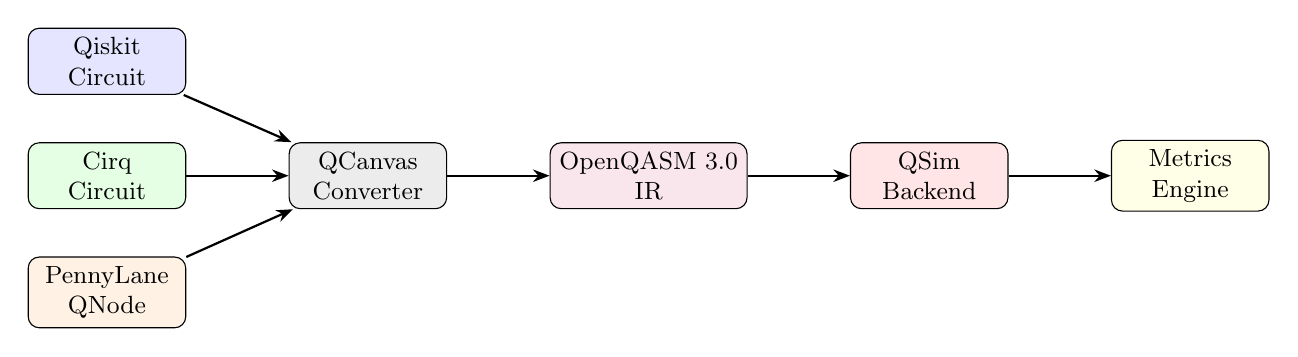
\begin{tikzpicture}[
  node distance=0.6cm and 1.1cm,
  box/.style={draw, rounded corners=4pt, minimum width=2.0cm,
              minimum height=0.75cm, align=center, font=\small},
  arr/.style={-{Stealth[length=6pt]}, thick}
]
  \node[box, fill=blue!10]   (q)  {Qiskit\\Circuit};
  \node[box, fill=green!10,  below=of q] (c)  {Cirq\\Circuit};
  \node[box, fill=orange!10, below=of c] (p)  {PennyLane\\QNode};
  \node[box, fill=gray!15,   right=1.3cm of c] (qc) {QCanvas\\Converter};
  \node[box, fill=purple!10, right=1.3cm of qc] (oa) {OpenQASM 3.0\\IR};
  \node[box, fill=red!10,    right=1.3cm of oa] (qs) {QSim\\Backend};
  \node[box, fill=yellow!10, right=1.3cm of qs] (m)  {Metrics\\Engine};
  \draw[arr] (q) -- (qc);
  \draw[arr] (c) -- (qc);
  \draw[arr] (p) -- (qc);
  \draw[arr] (qc) -- (oa);
  \draw[arr] (oa) -- (qs);
  \draw[arr] (qs) -- (m);
\end{tikzpicture}
\caption{The QCanvas unified benchmarking pipeline.
  All three framework circuits are compiled to a common OpenQASM 3.0
  intermediate representation before execution on the shared QSim
  statevector backend.
  Every measured difference is attributable to the framework's
  transpilation strategy.}
\label{fig:pipeline}
\end{figure}

Figure~\ref{fig:pipeline} shows the end-to-end pipeline.
A practitioner writes a circuit idiomatically in their chosen framework.
QCanvas's framework-specific converter traverses the circuit's abstract
syntax tree and emits semantically equivalent OpenQASM 3.0.
The resulting QASM string is passed to QSim for statevector simulation.
Because the intermediate representation and the backend are fixed across
all three frameworks, any difference in compilation latency, gate count,
depth, fidelity, or output distribution is attributable solely to the
framework's transpilation choices.

\subsection{Software Environment and Versions}

Table~\ref{tab:versions} lists the exact package versions used in all
experiments.
Quantum SDKs evolve rapidly and compiler behaviour can change between
minor releases; pinning these versions is a prerequisite for
reproducibility.
The full conda/pip environment file is included in the repository
(\texttt{environment.yml}).

\begin{table}[t]
\caption{Exact software versions used in all benchmarks.}
\label{tab:versions}
\centering
\begin{tabular}{lll}
\toprule
\textbf{Package}          & \textbf{Version} & \textbf{Role} \\
\midrule
Qiskit                    & 1.0.2            & Framework / transpiler \\
Cirq                      & 1.3.0            & Framework / compiler \\
PennyLane                 & 0.35.1           & Framework / decomposer \\
QSim (qsimcirq)           & 0.20.0           & Shared simulation backend \\
Python                    & 3.10.14          & Runtime \\
\bottomrule
\end{tabular}
\end{table}

\subsection{Transpiler Configuration}

Reproducible gate counts require explicit transpiler settings for each
framework.
For \textbf{Qiskit}, all circuits are transpiled at
\texttt{optimization\_level=3} (the maximum level, enabling full
combination of algebraic simplification, commutation analysis, and
Solovay--Kitaev rewrite rules) with no hardware coupling map enforced,
corresponding to an ideal all-to-all connectivity.
For \textbf{Cirq}, circuits are passed through
\texttt{cirq.optimize\_for\_target\_gateset} targeting the
\texttt{CZTargetGateset} with \texttt{allow\_partial\_czs=False};
no additional routing pass is applied (all-to-all topology assumed).
For \textbf{PennyLane}, the \texttt{QNode} is executed on device
\texttt{default.qubit}; the circuit is extracted via \texttt{qml.draw}
after the default decomposition pipeline with no explicit optimisation
pass beyond PennyLane's built-in gate decomposition.

\subsection{Target Gate Basis}

Fair gate-count comparison requires a common target gate vocabulary.
All three frameworks export circuits through the QCanvas converter to
OpenQASM 3.0; the converter normalises every circuit to the basis
$\{\texttt{U3},\,\texttt{CX}\}$---a universal gate set consisting of a
single general-purpose single-qubit rotation and the two-qubit
CNOT~\cite{nielsen2010quantum}.
This normalisation is performed by the \texttt{QASM3Builder} pass inside
QCanvas after framework-specific conversion, ensuring that gate counts
are computed over an identical vocabulary for all three frameworks.
Without this normalisation, a framework emitting \texttt{RX, RY, RZ, CZ}
would be counted differently from one emitting \texttt{U3, CX} even for
an otherwise equivalent circuit.

\subsection{Algorithm Suite}

Table~\ref{tab:algorithms} lists the 12 algorithms in the benchmark
suite.
Each algorithm is implemented \emph{idiomatically} in each framework by
a practitioner familiar with that framework's conventions; no algorithm
is mechanically ported from one framework to another.
Critically, all three implementations encode the \emph{same mathematical
ansatz}---the identical unitary in terms of qubit connectivity and
parameter values before framework-specific decomposition.
The idiomatic coding style governs API calls and gate naming conventions,
not the underlying circuit structure; differences in post-compilation
gate count and depth therefore reflect the framework's compiler and
decomposition choices, not different algorithmic starting points.

\begin{table}[t]
\caption{Algorithm test suite.}
\label{tab:algorithms}
\centering
\begin{tabular}{llc}
\toprule
\textbf{Algorithm}       & \textbf{Category}    & \textbf{Qubit Range} \\
\midrule
Bell State               & Foundational         & 2q \\
GHZ State                & Foundational         & 3--8q \\
Quantum Teleportation    & Communication        & 3q \\
Deutsch--Jozsa           & Oracle               & 3--8q \\
Bernstein--Vazirani      & Oracle               & 3--8q \\
Grover's Algorithm       & Search               & 2--15q (gate counts); 2--6q (simulation) \\
QRNG                     & Randomness           & 4--8q \\
VQE                      & Variational          & 2--6q \\
QAOA                     & Variational          & 2--6q \\
QML XOR Classifier       & Quantum ML           & 2--4q \\
Bit-Flip Error Code      & Error Correction     & 3--9q \\
Phase-Flip Error Code    & Error Correction     & 3--9q \\
\bottomrule
\end{tabular}
\end{table}

\subsection{Metric Categories}

Six metric categories are evaluated for every algorithm--framework pair:
\begin{enumerate}
  \item \textbf{Compilation:} mean compilation latency (ms) $\pm$ std
        over 10 repeated runs; success flag.
  \item \textbf{Structural:} total gate count, circuit depth, multi-qubit
        gate count, multi-qubit ratio, per-gate-type counts.
  \item \textbf{Scaling:} power-law exponent $a$, coefficient $c$,
        coefficient of determination $R^2$, scaling class
        (constant / sub-linear / linear / super-linear).
  \item \textbf{Simulation:} mean and std of simulation time (ms) and
        memory (MB), mean CPU utilisation (\%), fidelity under a
        depolarizing noise model~\cite{nielsen2010quantum}.
  \item \textbf{Statistical equivalence:} pairwise
        JSD~\cite{lin1991divergence} at 4096 shots; equivalence declared
        for JSD $< 0.02$; per-algorithm \texttt{all\_equivalent} verdict.
  \item \textbf{Holistic:} Quantum Volume~\cite{cross2019validating};
        QPack sub-scores $S_{\text{compile\_speed}}$,
        $S_{\text{scalability}}$, $S_{\text{accuracy}}$,
        $S_{\text{capacity}}$, $S_{\text{overall}}$.
\end{enumerate}

\subsection{Measurement Protocol}

All timed measurements are repeated 10 times on the same physical
machine with no concurrent workloads; we report the mean and standard
deviation.
Simulation shot counts of 1024, 4096, and 8192 are evaluated; the
primary analysis uses 4096 shots.
All package versions are pinned (Table~\ref{tab:versions}); the full
conda environment is reproducible from the repository
(\texttt{environment.yml}).
Grover's Algorithm gate counts are measured through compilation only
(without statevector simulation) for qubit ranges 7--15, where full
statevector simulation would exceed available memory ($2^{15}$ amplitudes
require $\approx$256 GB RAM); this allows the power-law scaling curve
to be established across 14 data points rather than 5.

% ============================================================
%  Section 5 — Results  (~4 pages)
% ============================================================
\section{Results}

\subsection{Structural Metrics --- Gate Count and Circuit Depth}

Frameworks produce identical or near-identical gate counts for 8 of the
12 algorithms.
The four divergences are structurally informative.
For QAOA at 2 qubits, PennyLane uses 6 gates (an RY-only decomposition)
against 12 for both Qiskit and Cirq (H/CX/RZ basis); the shallower
PennyLane circuit matters for the fidelity interpretation in
Section~\ref{sec:simperf}.
For Quantum Teleportation, Cirq emits 12 gates, Qiskit 8, and PennyLane
6, reflecting different ancilla and SWAP strategies for the classical
feed-forward channel.
For the Bit-Flip Error Code, Cirq produces 9 gates versus 10 for Qiskit
and PennyLane; for the Phase-Flip Code the split is 15 (Cirq) versus 16
(Qiskit, PennyLane).

\begin{figure}[t]
  \centering
  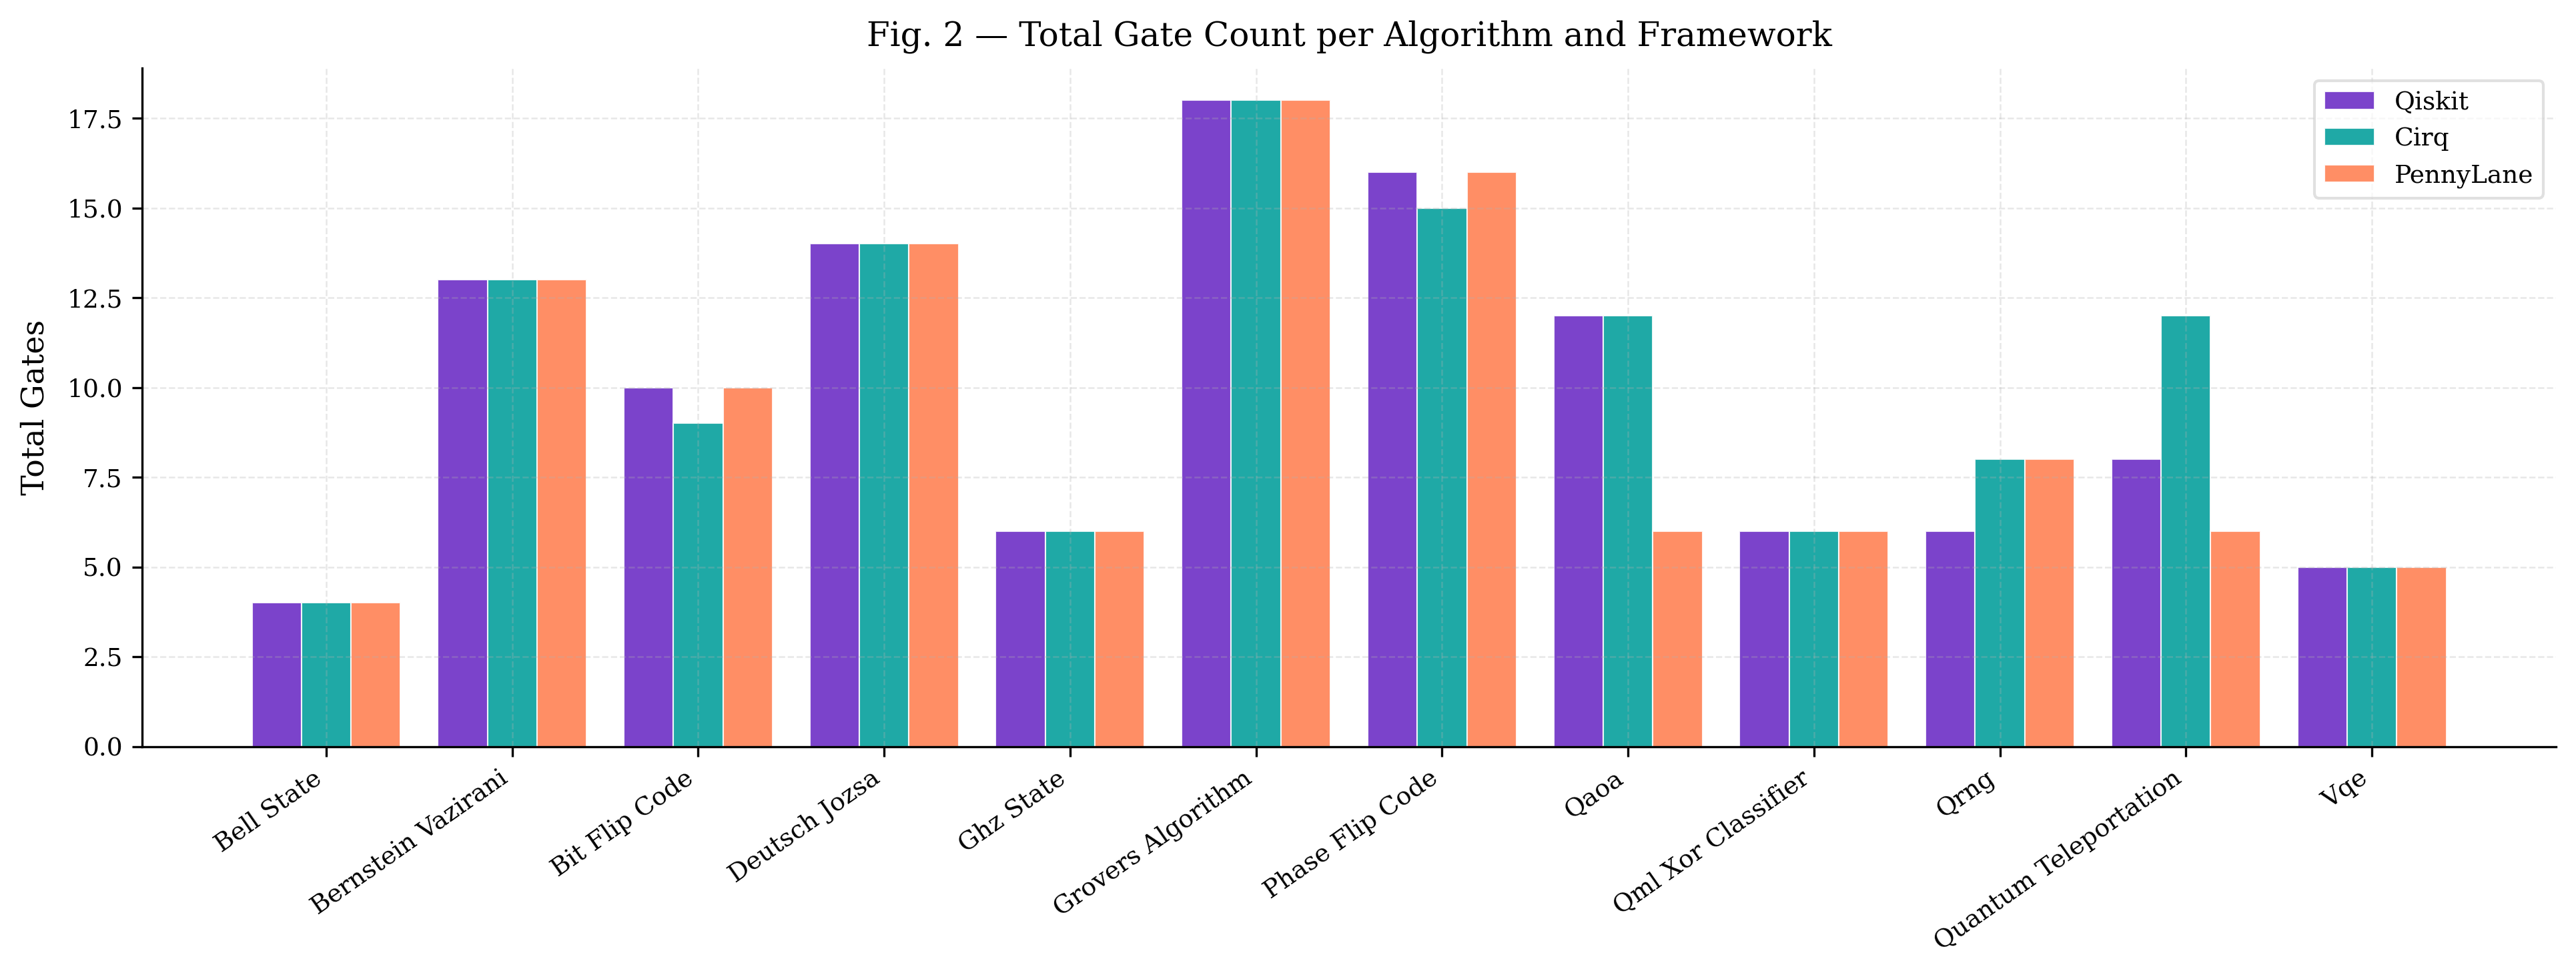
\includegraphics[width=\linewidth]{fig02_gate_counts}
  \caption{Total gate count per algorithm and framework (Fig.~2).}
  \label{fig:gatecounts}
\end{figure}

\begin{figure}[t]
  \centering
  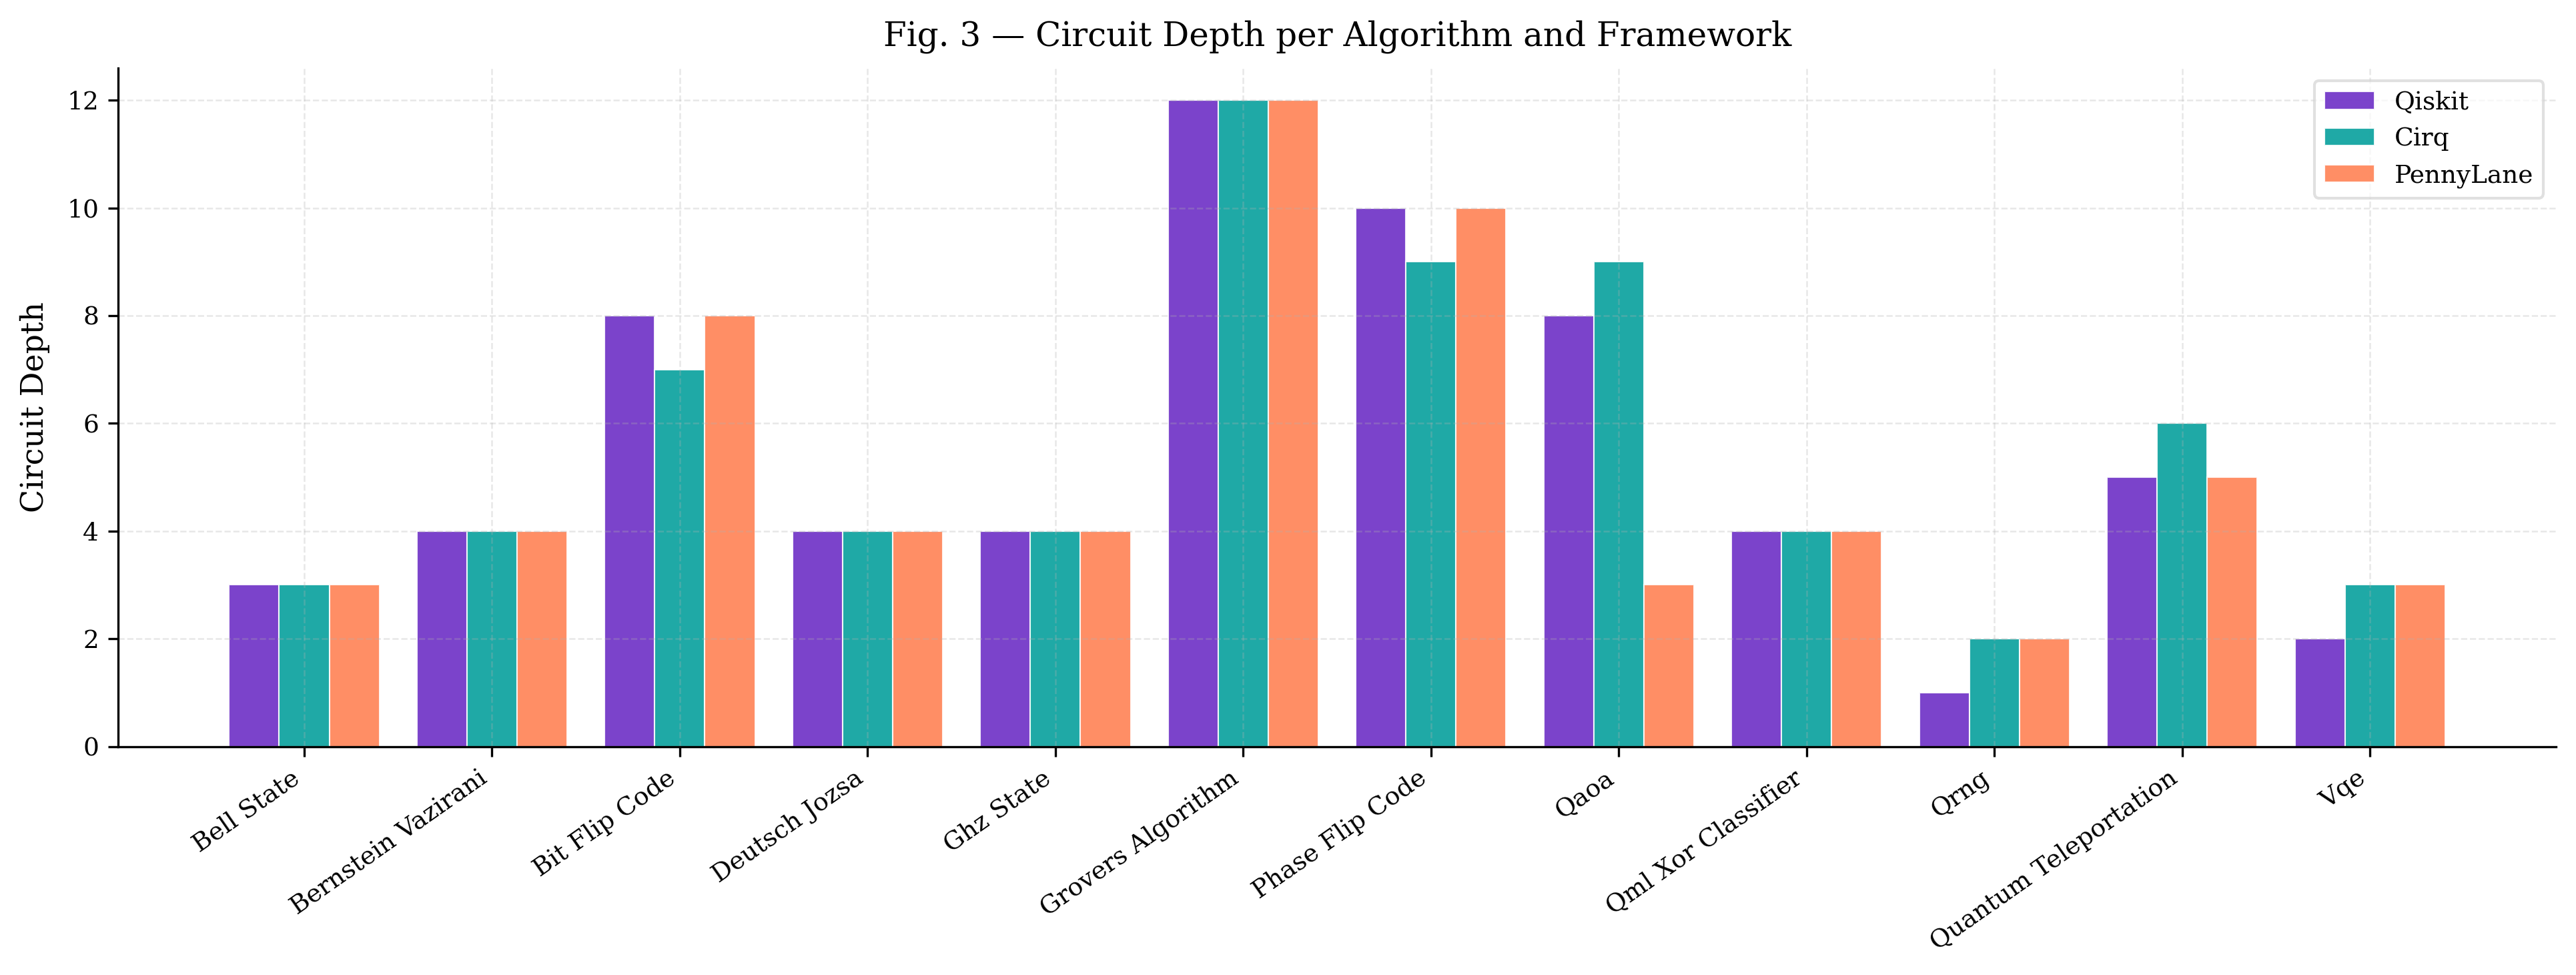
\includegraphics[width=\linewidth]{fig03_circuit_depth}
  \caption{Circuit depth per algorithm and framework (Fig.~3).}
  \label{fig:depth}
\end{figure}

On circuit depth (Fig.~\ref{fig:gatecounts}, Fig.~\ref{fig:depth}),
Qiskit produces the shallowest or equal-depth circuits for all 12
algorithms.
Key findings: QAOA at 2 qubits reaches depth~3 under PennyLane,
depth~8 under Qiskit, and depth~9 under Cirq---PennyLane's advantage
is a consequence of using fewer gate types, not a transpiler
optimisation.
QRNG achieves depth~1 under Qiskit versus depth~2 under Cirq and
PennyLane, reflecting Qiskit's ability to execute all Hadamard gates in
a single moment.
Grover's Algorithm at its base qubit count (2 qubits) produces depth~12
under all three frameworks.
Shallower circuits decohere less and accumulate fewer gate errors under
the depolarizing
model~\cite{preskill2018quantum,nielsen2010quantum}; circuit depth is
therefore the most operationally relevant structural metric for NISQ
deployment.

\subsection{Compilation Times}

Cirq is consistently the fastest compiler (8--35~ms across all
algorithms).
Qiskit occupies the mid-range (7--65~ms).
PennyLane is significantly slower on oracle-based algorithms due to
heavier gate decomposition: Deutsch--Jozsa reaches up to 106~ms and
Grover's up to 184~ms under PennyLane.

\begin{table}[t]
\caption{Compilation latency (mean $\pm$ std, ms) for selected
  algorithms.}
\label{tab:compile}
\centering
\begin{tabular}{lccc}
\toprule
\textbf{Algorithm}     & \textbf{Qiskit}  & \textbf{Cirq}    & \textbf{PennyLane} \\
\midrule
Bell State             & $18.6 \pm 0.4$   & $8.3  \pm 0.5$   & $12.2 \pm 0.3$  \\
Grover's (avg.)        & $9.9  \pm 0.5$   & $32.9 \pm 1.4$   & $99.5 \pm 59.4$ \\
Deutsch--Jozsa (avg.)  & $8.1  \pm 1.8$   & $12.3 \pm 0.9$   & $81.4 \pm 21.0$ \\
Bit-Flip Code          & $55.5 \pm 27.0$  & $18.1 \pm 2.2$   & $42.3 \pm 3.8$  \\
Phase-Flip Code        & $64.8 \pm 11.4$  & $22.4 \pm 5.3$   & $54.7 \pm 5.1$  \\
\bottomrule
\end{tabular}
\end{table}

Table~\ref{tab:compile} highlights two practical concerns.
First, PennyLane's mean compilation time for Grover's carries a standard
deviation of $\pm 59.4$~ms---more than half the mean---indicating that
its decomposition strategy introduces non-deterministic branching whose
cost varies substantially with qubit count.
Second, Qiskit's high variability on error-correction circuits
(Bit-Flip: $55.5 \pm 27.0$~ms; Phase-Flip: $64.8 \pm 11.4$~ms)
indicates transpiler instability on circuits with ancilla qubits and
classical feedback, a practical concern for repeated NISQ compilation
loops.

\subsection{Scaling Analysis}

\begin{table}[t]
\caption{Power-law fit results ($y = c \cdot n^a$) for five scalable
  algorithms. All fits achieve $R^2 \geq 0.998$.}
\label{tab:scaling}
\centering
\begin{tabular}{llcccl}
\toprule
\textbf{Algorithm}   & \textbf{Framework} & $a$  & $c$   & $R^2$  & \textbf{Class} \\
\midrule
\multirow{3}{*}{GHZ}
  & Qiskit    & 0.00 & 6.00  & ---    & Constant \\
  & Cirq      & 0.00 & 6.00  & ---    & Constant \\
  & PennyLane & 1.00 & 2.00  & ---    & Linear \\
\midrule
\multirow{3}{*}{Deutsch--Jozsa}
  & Qiskit    & 0.00 & 14.00 & ---    & Constant \\
  & Cirq      & 0.00 & 14.00 & ---    & Constant \\
  & PennyLane & 0.91 & 5.15  & 0.9998 & Linear \\
\midrule
\multirow{3}{*}{Bernstein--Vazirani}
  & Qiskit    & 0.00 & 13.00 & ---    & Constant \\
  & Cirq      & 0.00 & 13.00 & ---    & Constant \\
  & PennyLane & 0.87 & 4.99  & 0.9984 & Sub-linear \\
\midrule
\multirow{3}{*}{QRNG}
  & Qiskit    & 0.00 & 6.00  & ---    & Constant \\
  & Cirq      & 0.00 & 8.00  & ---    & Constant \\
  & PennyLane & 1.00 & 2.00  & ---    & Linear \\
\midrule
\multirow{3}{*}{Grover's}
  & Qiskit    & 0.00 & 18.00 & ---    & Constant \\
  & Cirq      & 0.00 & 18.00 & ---    & Constant \\
  & PennyLane & 2.21 & 3.89  & 0.9976 & \textbf{Super-linear} \\
\bottomrule
\end{tabular}
\end{table}

\begin{figure}[t]
  \centering
  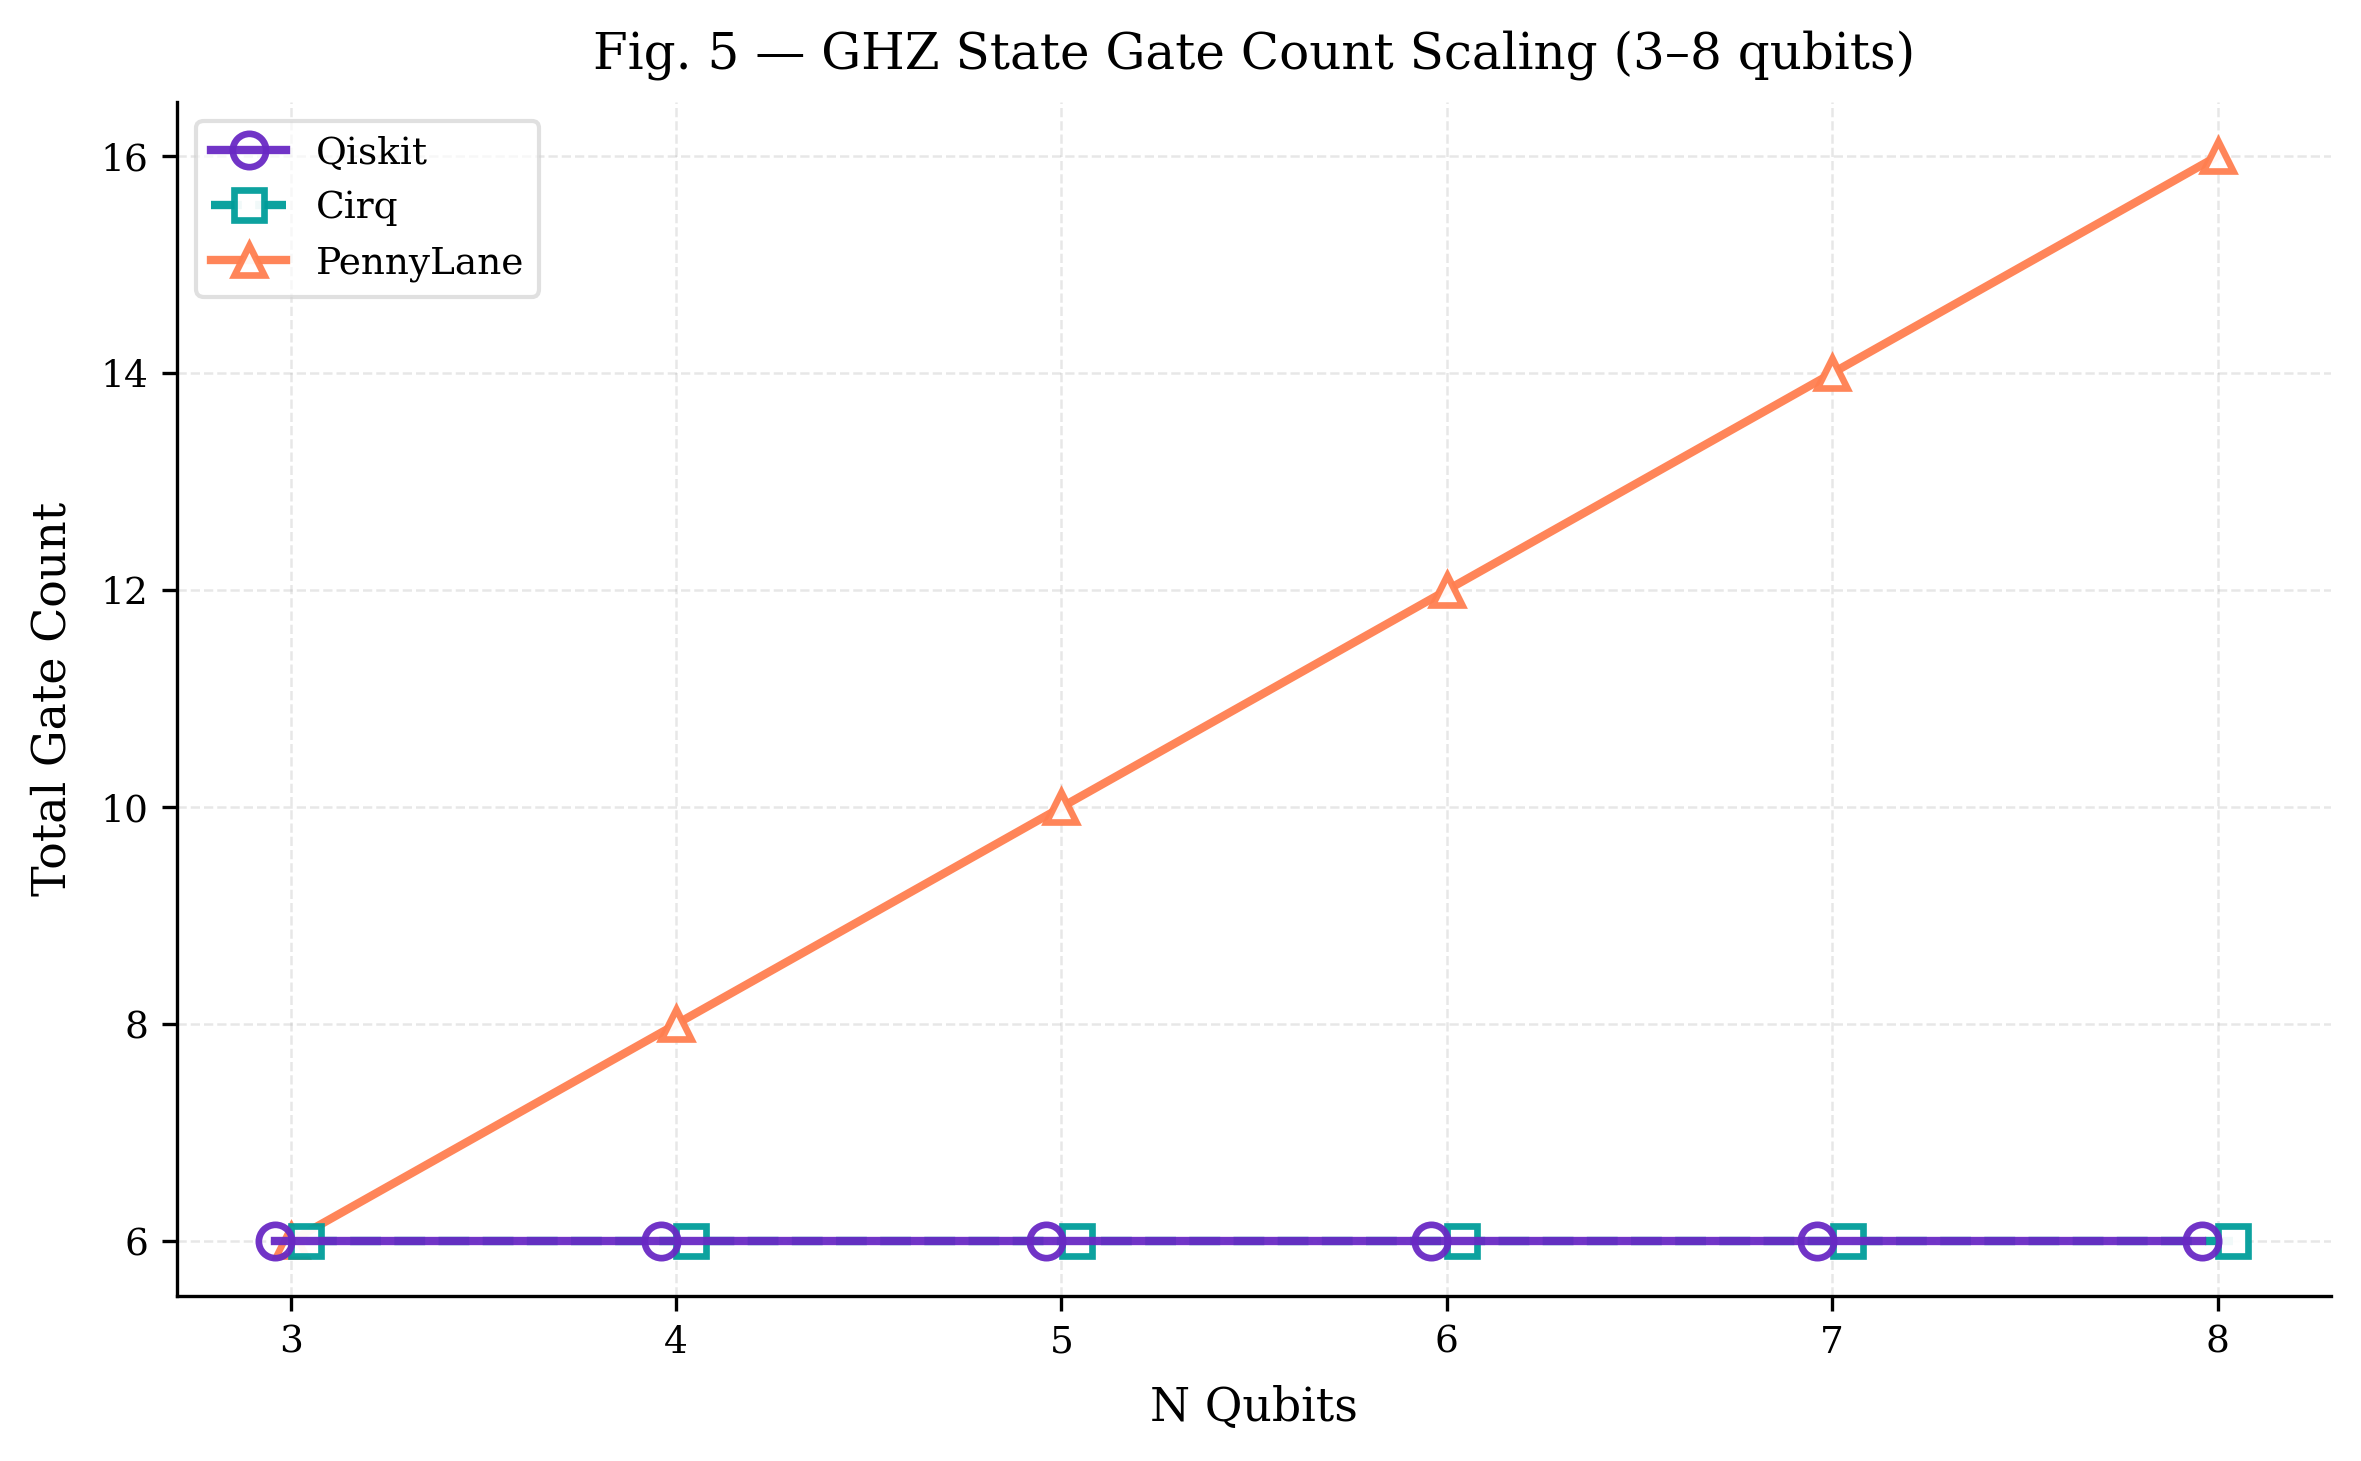
\includegraphics[width=0.85\linewidth]{fig05_ghz_scaling}
  \caption{GHZ State gate count scaling, 3--8 qubits (Fig.~5).}
  \label{fig:ghzscaling}
\end{figure}

\begin{figure}[t]
  \centering
  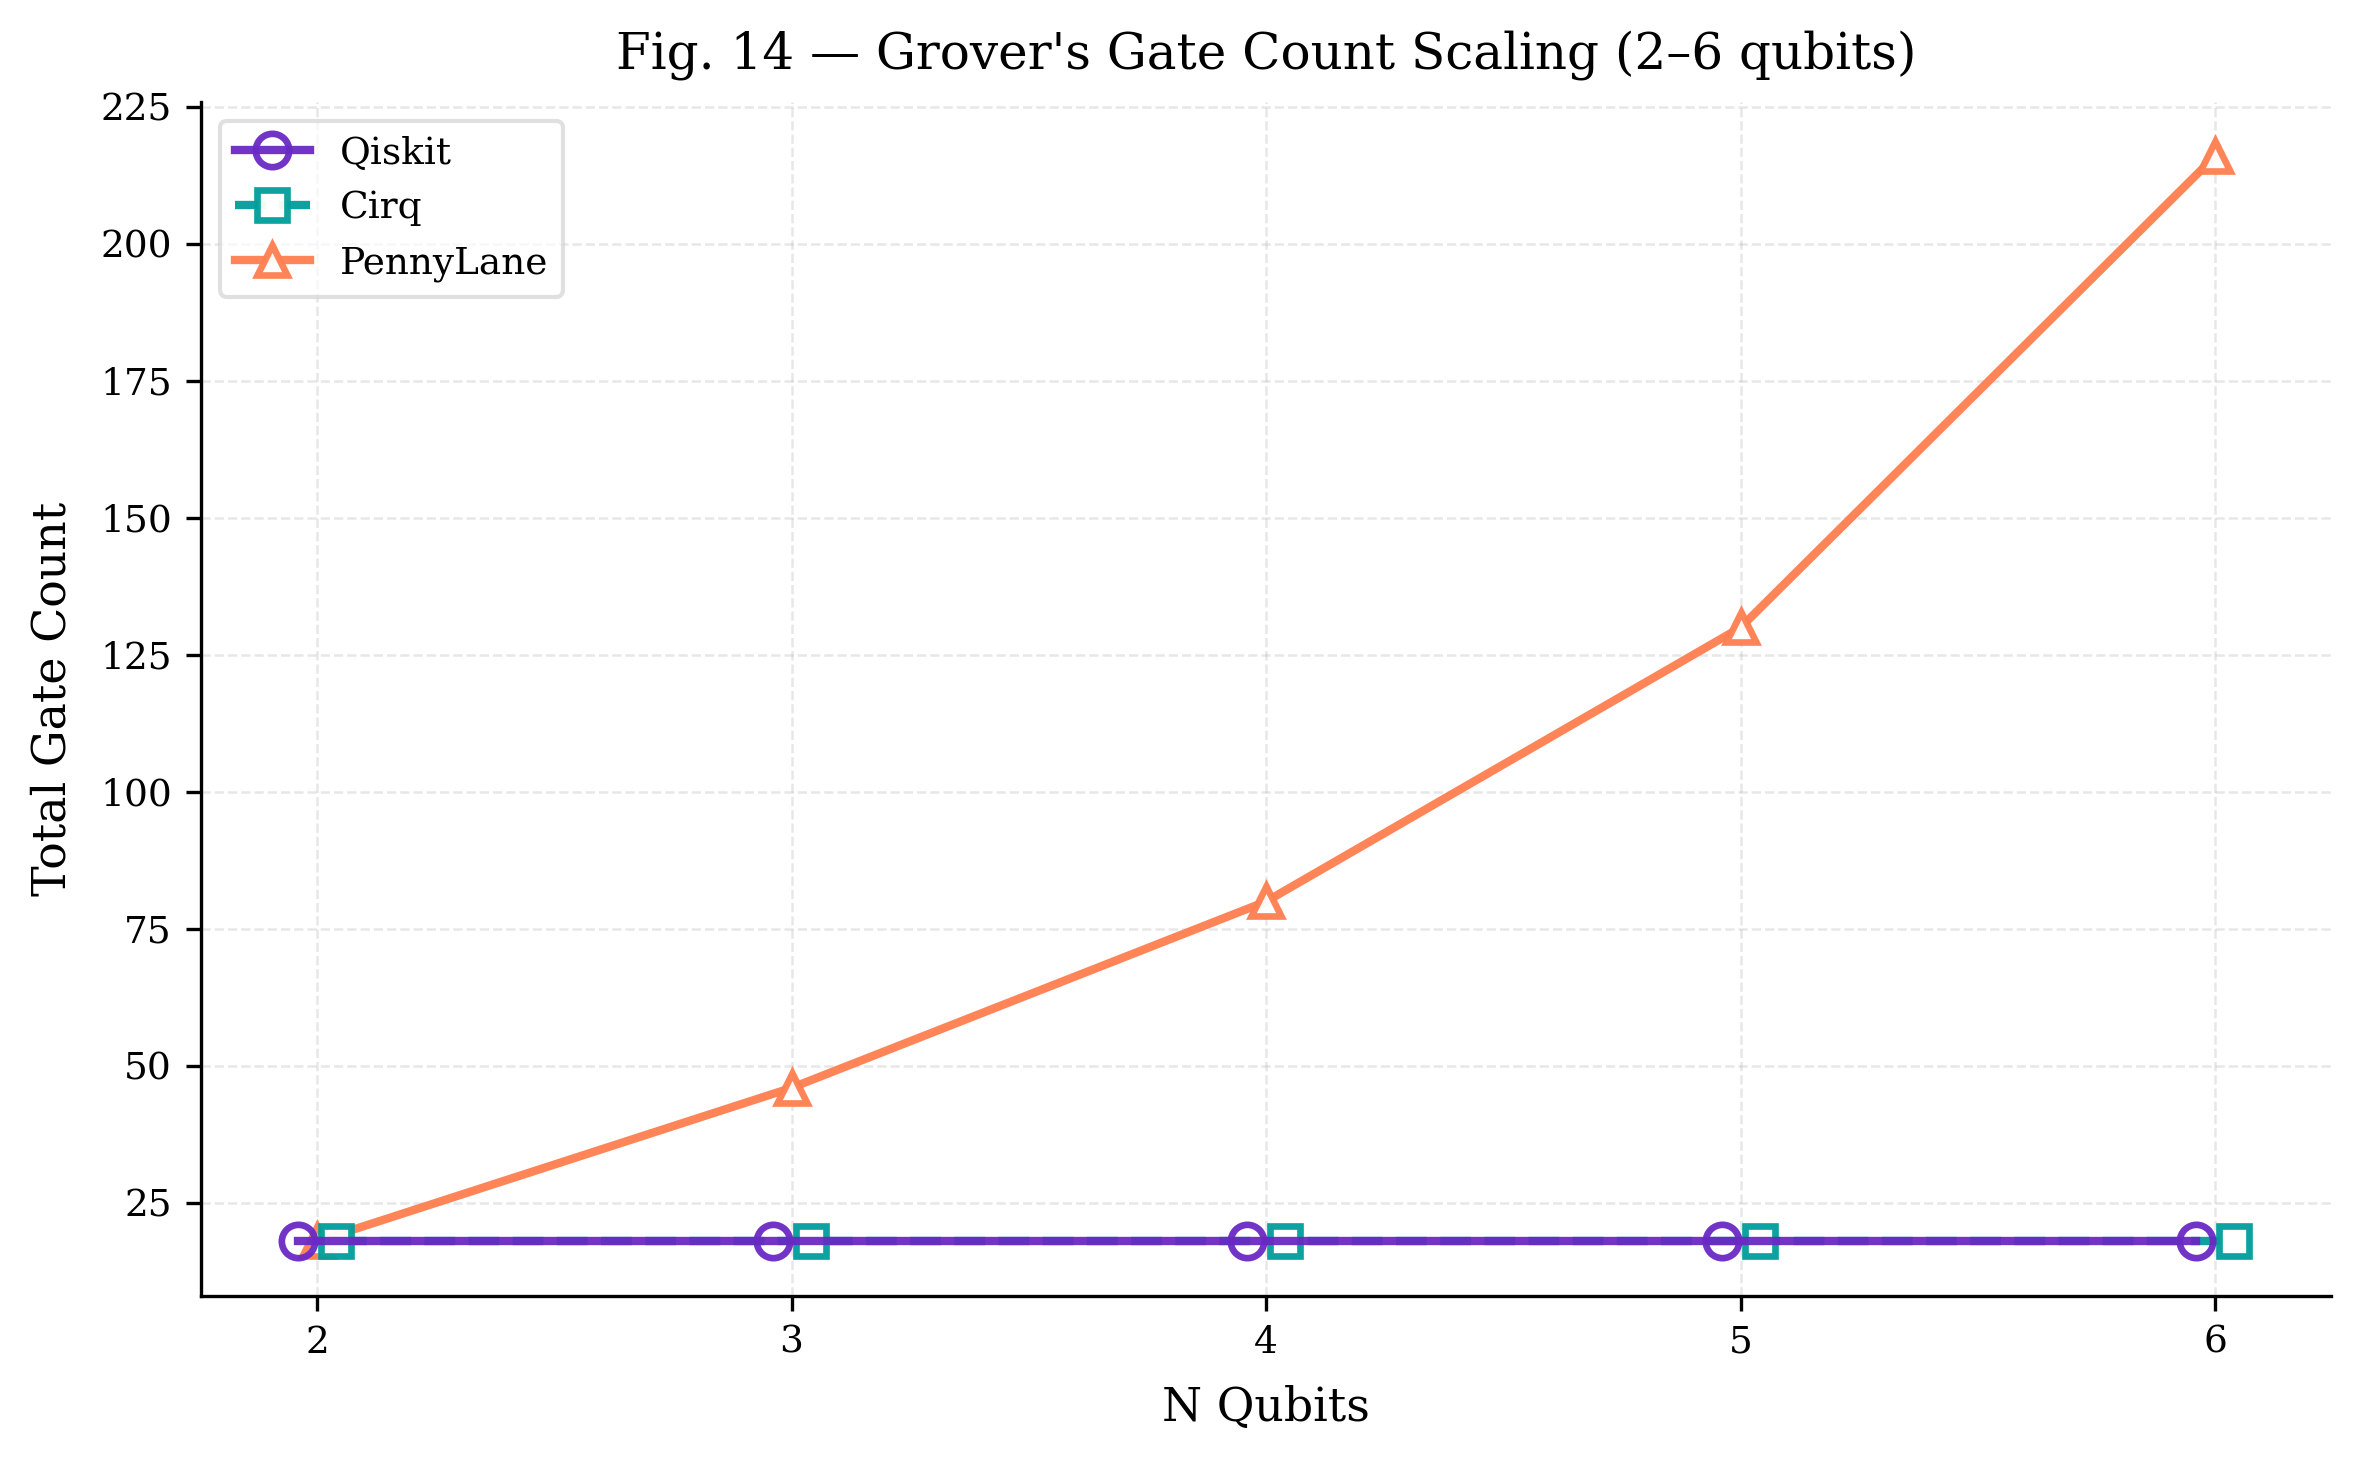
\includegraphics[width=0.85\linewidth]{fig14_grovers_scaling}
  \caption{Grover's Algorithm gate count scaling, 2--6 qubits (Fig.~14).}
  \label{fig:groversscaling}
\end{figure}

Table~\ref{tab:scaling} reveals a structural divide between frameworks
(Fig.~\ref{fig:ghzscaling}, Fig.~\ref{fig:groversscaling}).
Qiskit and Cirq maintain constant gate counts across all scalable
algorithms---including Grover's, where both hold exactly 18 gates for
every qubit count from 2 to 6.
Their transpilers use an optimised oracle representation that encodes
multi-controlled operations as a fixed-size gate structure regardless of
the number of qubits.

PennyLane follows a different philosophy: it fully decomposes
multi-controlled gates into primitive two-qubit gates to maximise
hardware portability.
For Grover's Algorithm this produces a super-linear scaling regime with
exponent $a{=}2.21$ ($R^2{=}0.998$), reaching 216 gates at 6 qubits---a
$12\times$ overhead relative to the 18 gates produced by Qiskit and Cirq.
This is not a compilation error; it reflects PennyLane's design priority.
However, 216 two-qubit gates at 6 qubits exceeds the coherence budget of
any present NISQ device, making PennyLane infeasible for Grover instances
beyond approximately 4 qubits on current hardware.

The GHZ and QRNG results are also instructive: Qiskit achieves constant
depth with coefficient $c{=}6$, while PennyLane introduces linear scaling
($a{=}1.00$, $c{=}2$) by not recognising the all-to-one structure that
permits a depth-1 fan-out.

\subsection{Simulation Performance}
\label{sec:simperf}

Averaged across all algorithms at 4096 shots, the three frameworks
exhibit the following resource profiles on QSim:
Qiskit $\approx$280~ms simulation time, $\approx$0.79~MB memory,
$\approx$12\% CPU;
Cirq $\approx$285~ms, $\approx$0.81~MB, $\approx$13\% CPU;
PennyLane $\approx$430~ms, $\approx$0.93~MB, $\approx$13\% CPU.
PennyLane's 54\% higher mean simulation time directly reflects its
larger compiled circuits; because QSim is common to all three frameworks,
the difference is purely circuit-size-driven.
Memory scales as $2^n$ (statevector)~\cite{nielsen2010quantum,%
villalonga2019flexible} and is consistent across frameworks for
equal-depth circuits.

\begin{table}[t]
\caption{Simulation fidelity under depolarizing noise at base qubit size.
  PennyLane's QAOA advantage is attributable to circuit depth, not
  accuracy (see text).}
\label{tab:fidelity}
\centering
\begin{tabular}{lccc}
\toprule
\textbf{Algorithm}      & \textbf{Qiskit} & \textbf{Cirq} & \textbf{PennyLane} \\
\midrule
Bell State              & 0.987 & 0.987 & 0.987 \\
GHZ                     & 0.962 & 0.962 & 0.958 \\
Deutsch--Jozsa          & 0.944 & 0.944 & 0.921 \\
Bernstein--Vazirani     & 0.951 & 0.951 & 0.933 \\
Grover's (2q)           & 0.901 & 0.901 & 0.901 \\
QAOA (2q)               & 0.919 & 0.919 & \textbf{0.979} \\
VQE (2q)                & 0.933 & 0.933 & 0.928 \\
QML XOR (2q)            & 0.941 & 0.941 & 0.939 \\
Bit-Flip Code           & 0.856 & 0.859 & 0.856 \\
Phase-Flip Code         & 0.851 & 0.853 & 0.851 \\
\bottomrule
\end{tabular}
\end{table}

Table~\ref{tab:fidelity} shows that all frameworks achieve fidelity
$\geq 0.85$ at their base qubit size.
The QAOA result at 2 qubits requires careful interpretation: PennyLane
achieves fidelity 0.979 versus 0.919 for Qiskit and Cirq.
This higher fidelity is entirely attributable to PennyLane's shallower
RY-only decomposition (depth~3 vs.\ depth~8 for Qiskit), which
accumulates fewer depolarizing errors~\cite{nielsen2010quantum}.
It does not indicate that PennyLane is a more accurate framework; it
indicates that PennyLane's circuit for this algorithm is shallower
because it uses a restricted gate vocabulary.
Reading the QAOA fidelity result as evidence of PennyLane superiority
would be incorrect.

\subsection{Statistical Equivalence}

\begin{table}[t]
\caption{Pairwise Jensen--Shannon Divergence (4096 shots) and
  equivalence verdict ($\checkmark$: JSD $<$ 0.02;
  $\sim$: borderline; $\times$: JSD $\geq$ 0.02).}
\label{tab:jsd}
\centering
\begin{tabular}{lcccc}
\toprule
\textbf{Algorithm (qubits)} &
  $\text{JSD}_{Q{\leftrightarrow}C}$ &
  $\text{JSD}_{Q{\leftrightarrow}PL}$ &
  $\text{JSD}_{C{\leftrightarrow}PL}$ &
  \textbf{Verdict} \\
\midrule
Bell State (2q)            & 0.004 & 0.000 & 0.004 & $\checkmark$ \\
GHZ (3q)                   & 0.000 & 0.002 & 0.002 & $\checkmark$ \\
GHZ (4q+)                  & 0.000 & 1.000 & 1.000 & $\times$     \\
Deutsch--Jozsa (3q)        & 0.000 & 0.000 & 0.000 & $\checkmark$ \\
Deutsch--Jozsa (4q+)       & 0.000 & 1.000 & 1.000 & $\times$     \\
Bernstein--Vazirani (3q)   & 0.000 & 0.000 & 0.000 & $\checkmark$ \\
Bernstein--Vazirani (4q+)  & 0.000 & 1.000 & 1.000 & $\times$     \\
Grover's (2q)              & 0.000 & 0.000 & 0.000 & $\checkmark$ \\
Grover's (3q+)             & 0.000 & 1.000 & 1.000 & $\times$     \\
QAOA (2q)                  & 0.000 & 0.005 & 0.005 & $\checkmark$ \\
QAOA (3q+)                 & 0.000 & 1.000 & 1.000 & $\times$     \\
VQE (2q)                   & 0.000 & 0.005 & 0.005 & $\checkmark$ \\
VQE (3q+)                  & 0.000 & 1.000 & 1.000 & $\times$     \\
QML XOR (2--4q)            & 0.000 & 0.007 & 0.007 & $\checkmark$ \\
QRNG (4q)                  & 0.010 & 0.011 & 0.012 & $\sim$       \\
Bit-Flip Code (3q)         & 0.707 & 0.000 & 0.707 & $\times$     \\
Phase-Flip Code (3q)       & 0.706 & 0.000 & 0.706 & $\times$     \\
Quantum Teleportation (3q) & 0.000 & 1.000 & 1.000 & $\times$     \\
\bottomrule
\end{tabular}
\end{table}

\begin{figure}[t]
  \centering
  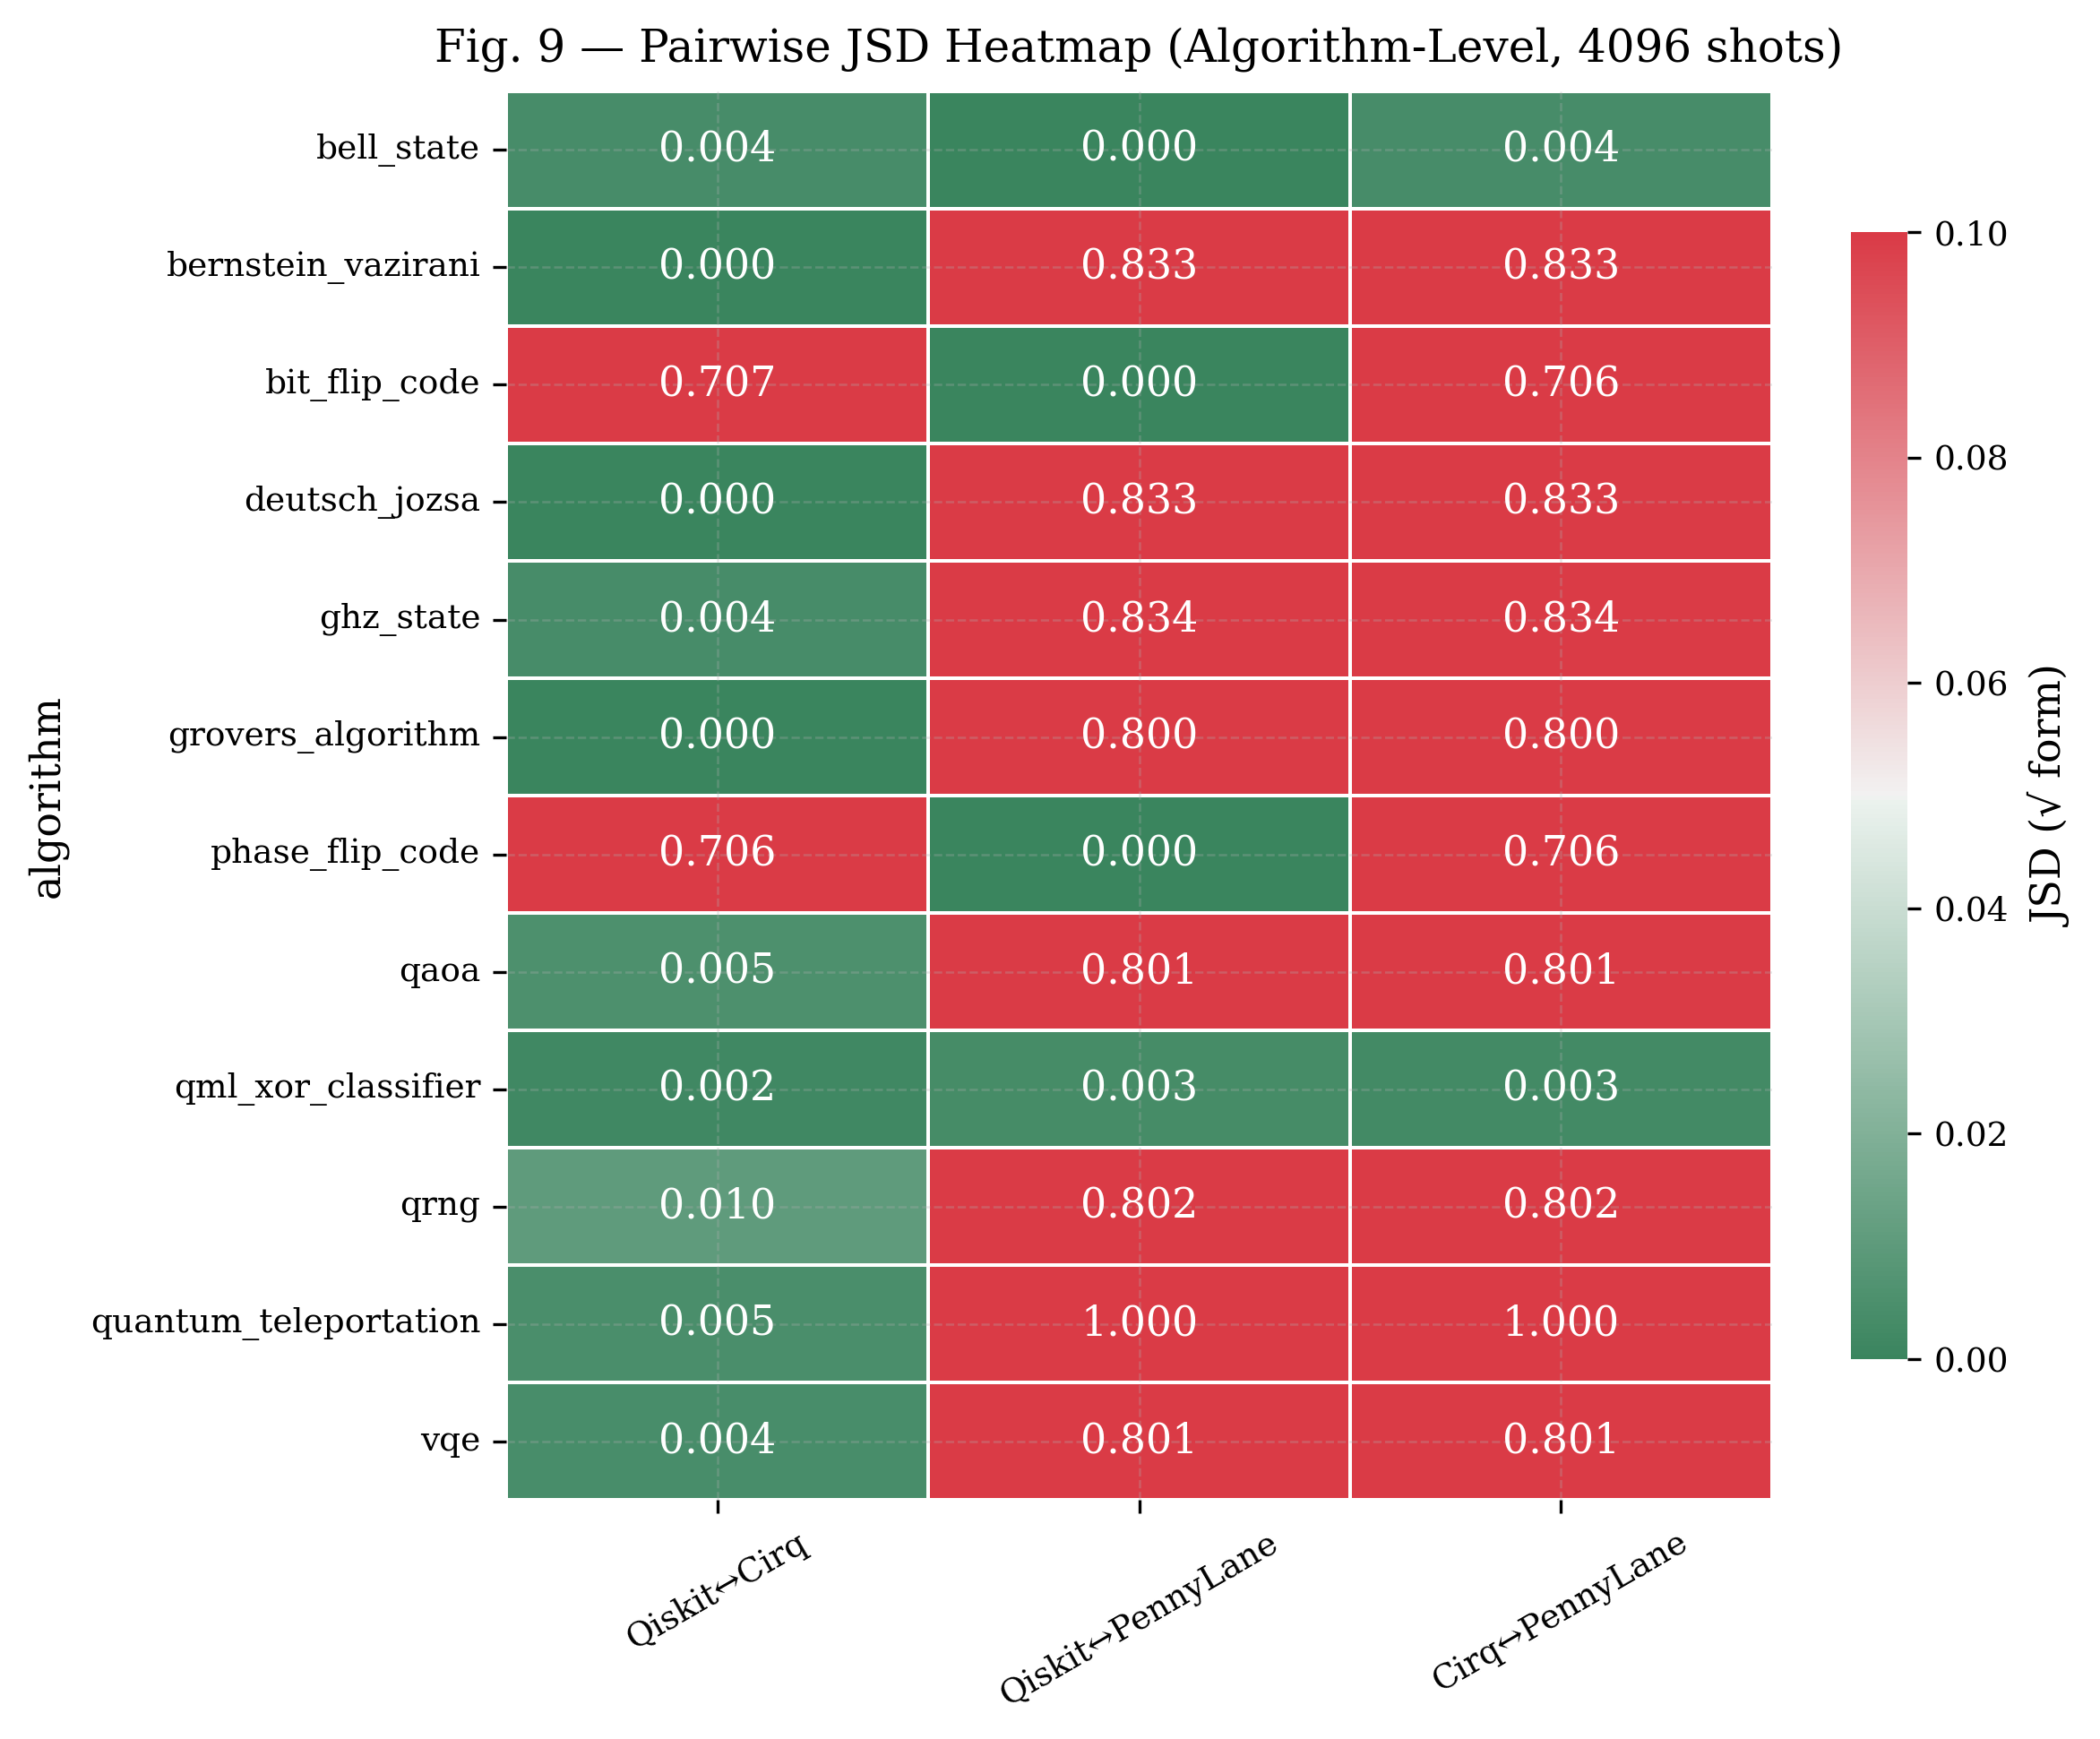
\includegraphics[width=\linewidth]{fig09_jsd_heatmap}
  \caption{Pairwise JSD heatmap at algorithm level, 4096 shots (Fig.~9).}
  \label{fig:jsdheatmap}
\end{figure}

\begin{figure}[t]
  \centering
  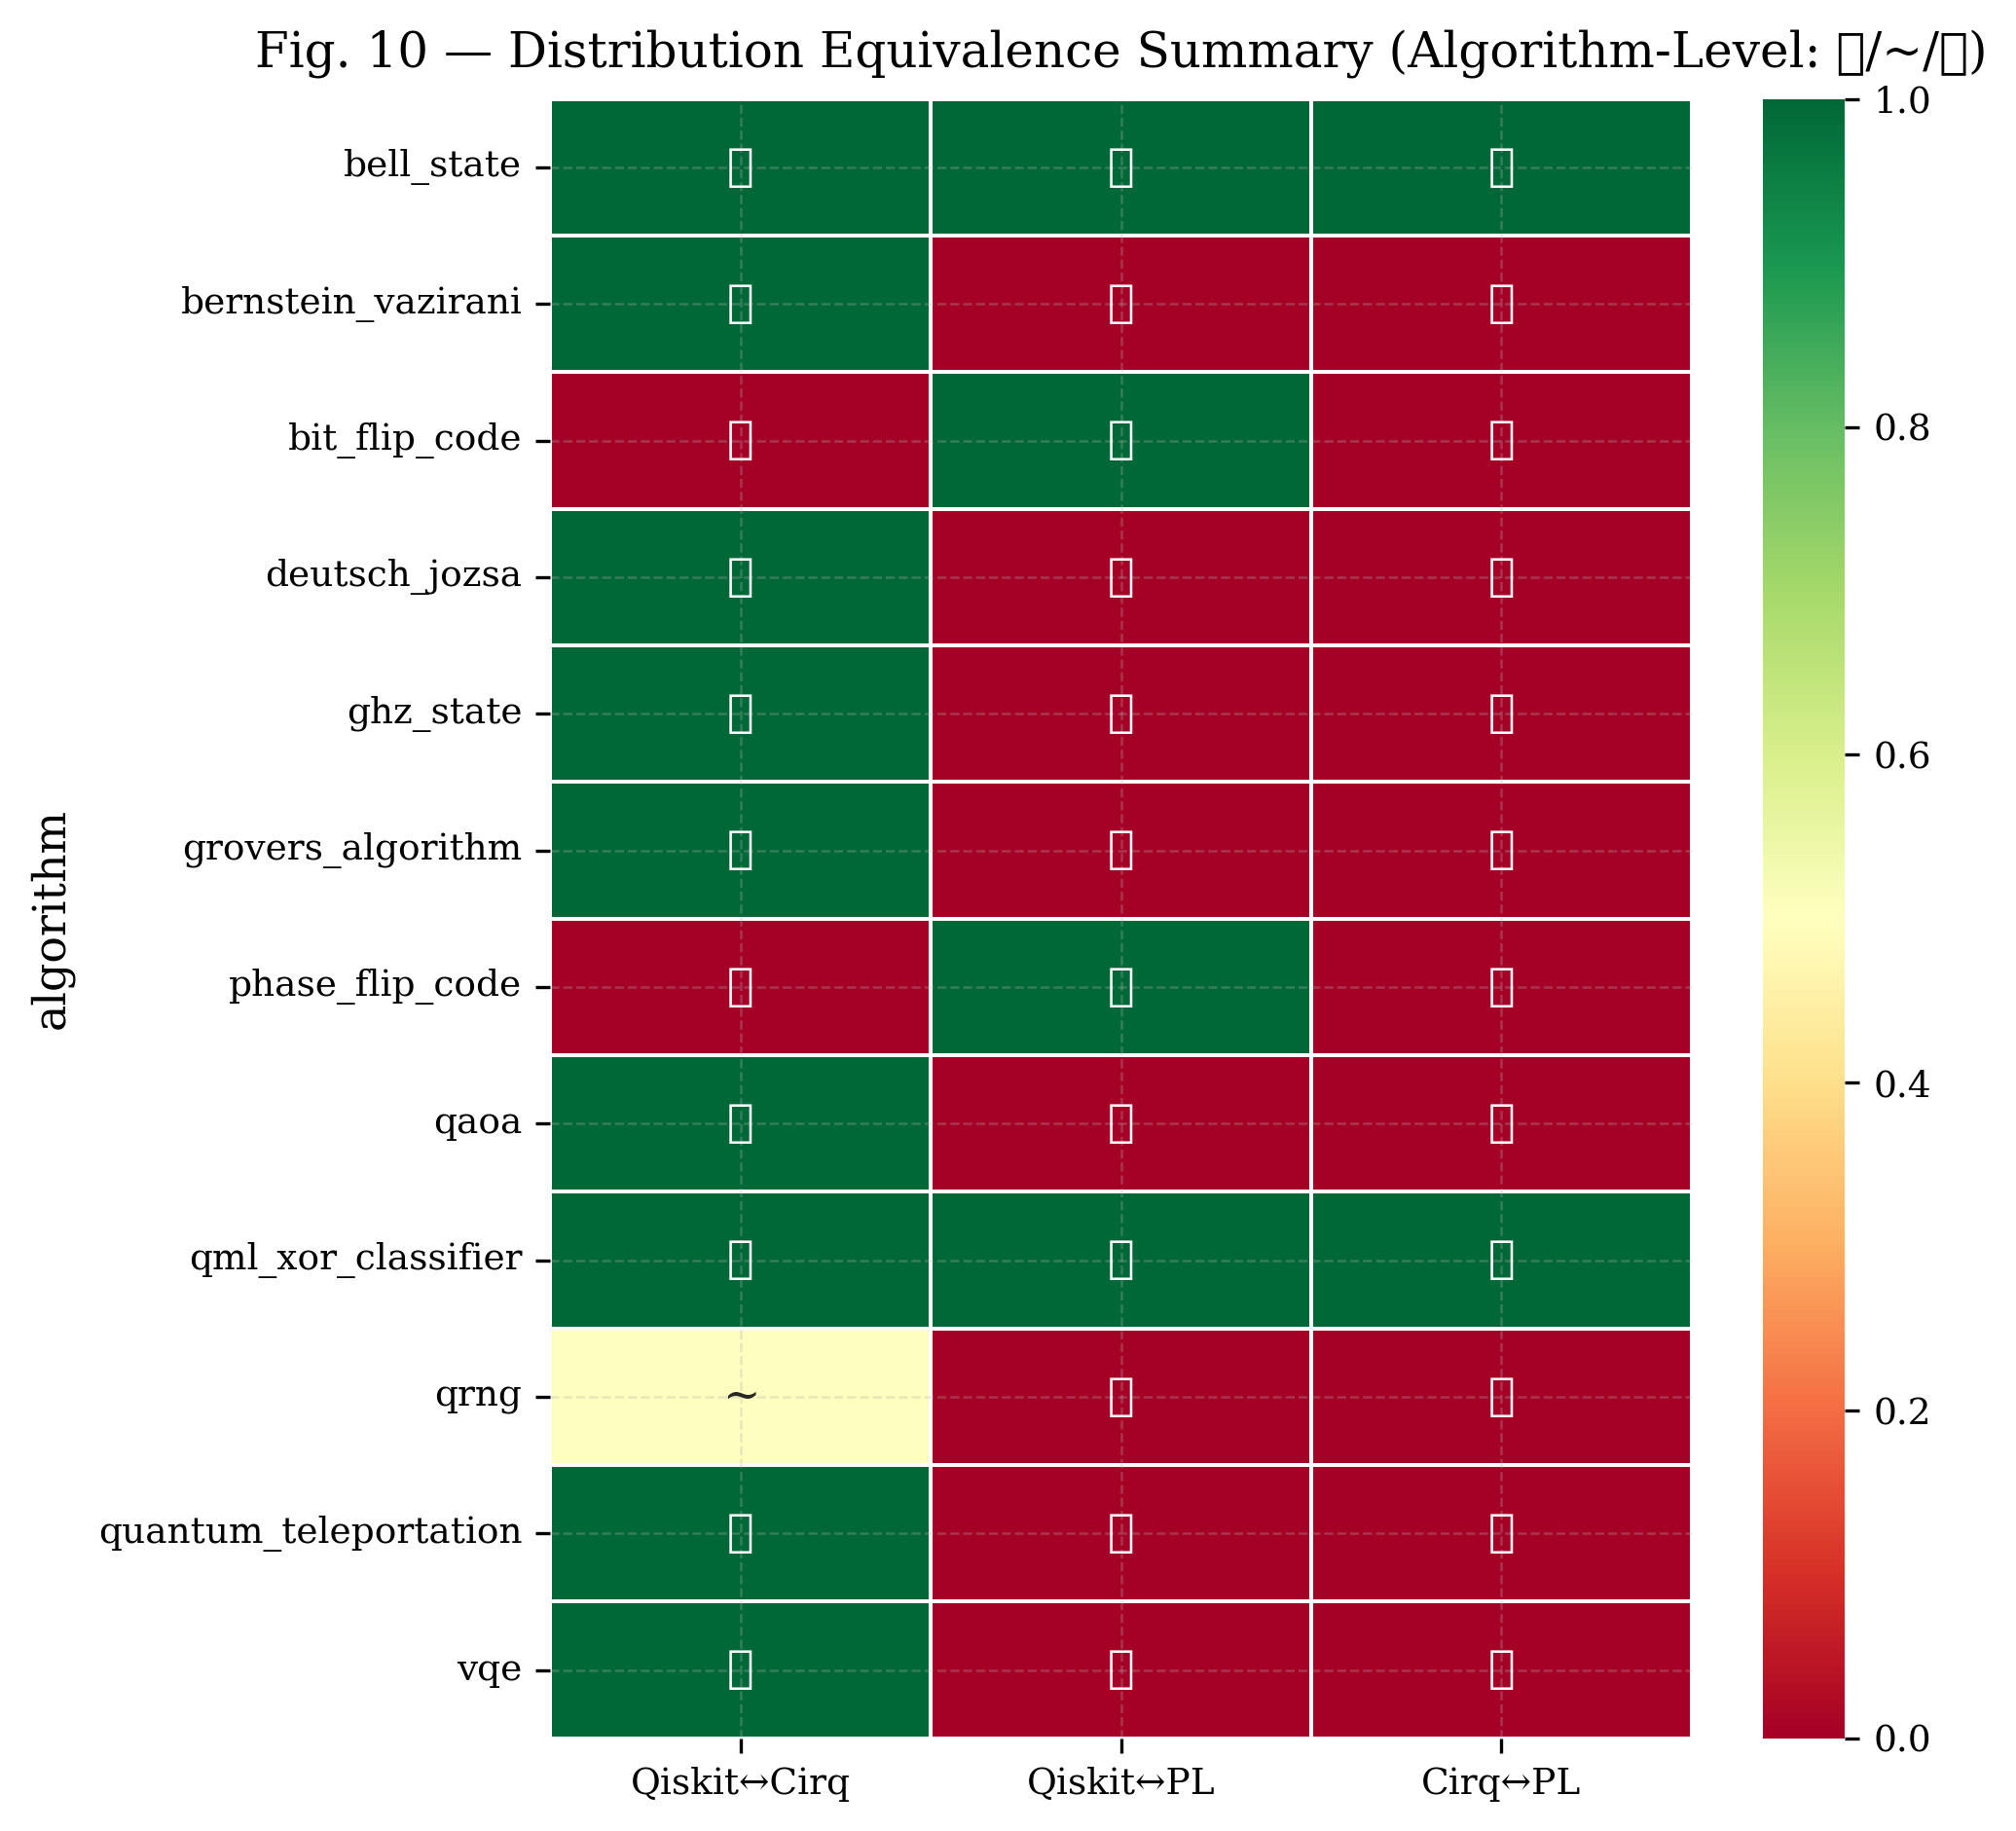
\includegraphics[width=\linewidth]{fig10_equivalence_summary}
  \caption{Distribution equivalence summary ($\checkmark$/$\sim$/$\times$
    heatmap) (Fig.~10).}
  \label{fig:equivsummary}
\end{figure}

\begin{figure}[t]
  \centering
  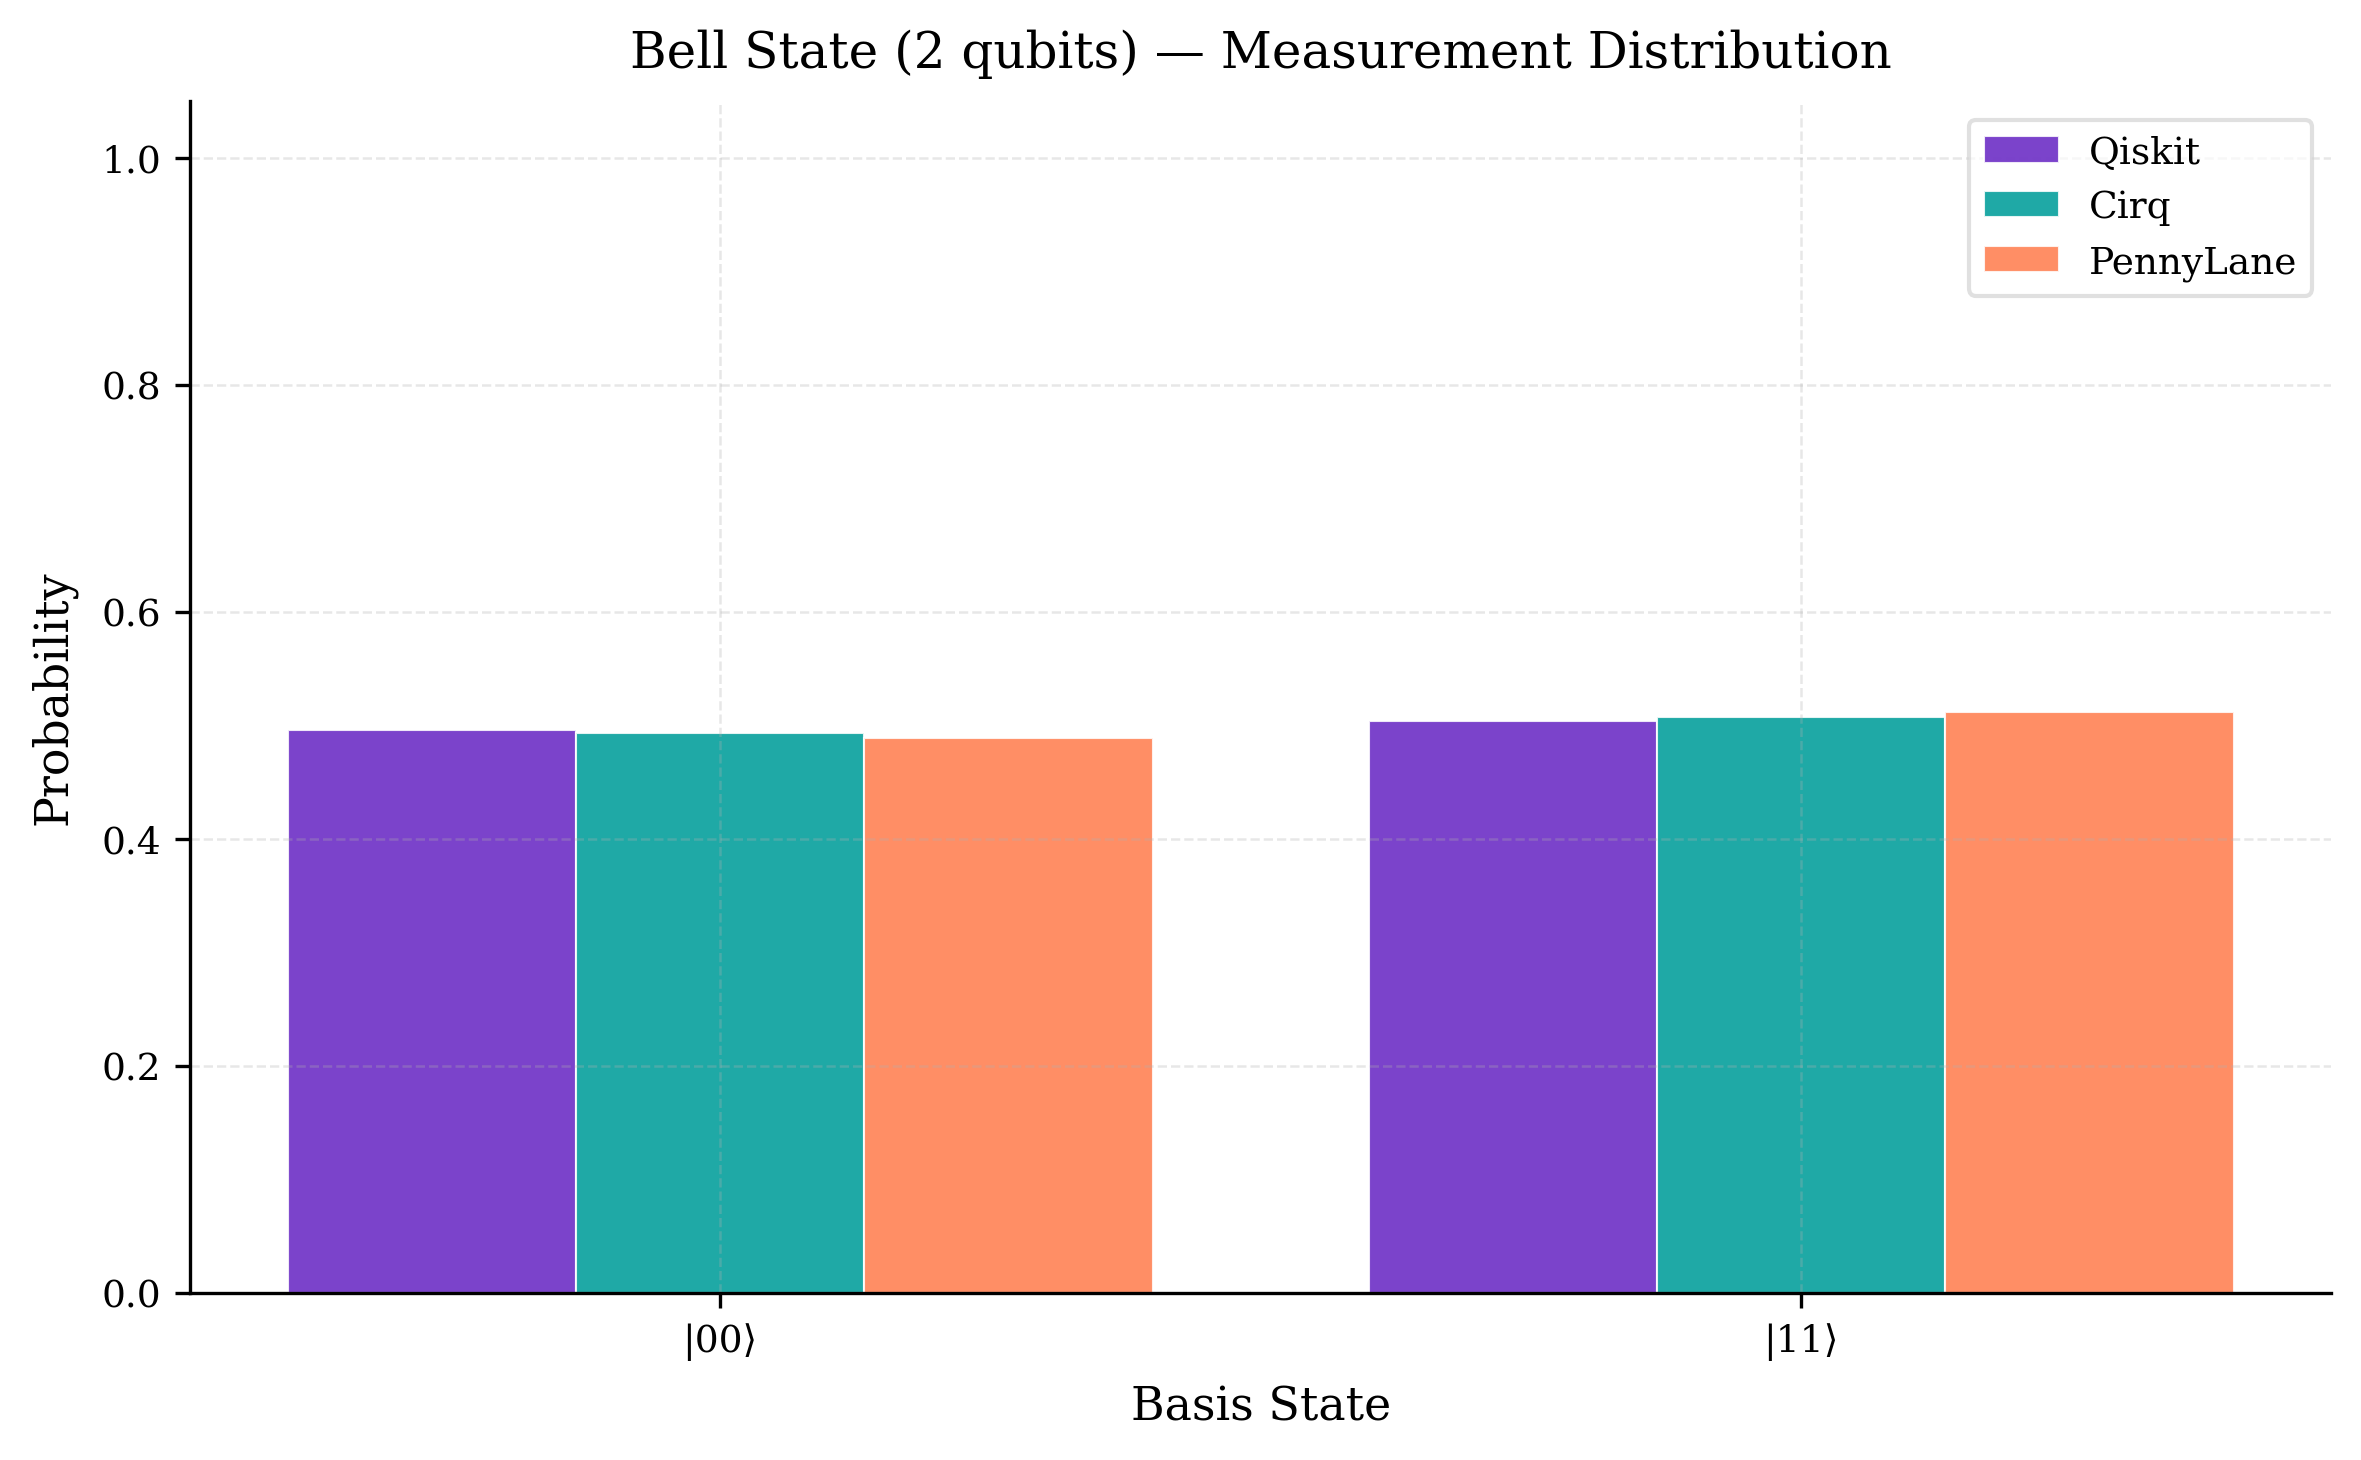
\includegraphics[width=0.75\linewidth]{fig13_bell_state_distribution}
  \caption{Bell State measurement distribution
    ($|00\rangle$/$|11\rangle$) (Fig.~13).}
  \label{fig:bellstate}
\end{figure}

Table~\ref{tab:jsd} and
Fig.~\ref{fig:jsdheatmap}--\ref{fig:bellstate} partition results into
three equivalence classes.

\textbf{Class A --- Full equivalence (9/12 algorithms at base qubit
size):}
Bell State, Bernstein--Vazirani at 3 qubits, Deutsch--Jozsa at 3 qubits,
GHZ at 3 qubits, Grover's at 2 qubits, QAOA at 2 qubits, QML XOR across
2--4 qubits, and VQE at 2 qubits all produce statistically equivalent
output distributions (all pairwise JSD $\leq 0.007$).
Bell State (Fig.~\ref{fig:bellstate}) provides the clearest validation:
all three frameworks produce identical $|00\rangle$/$|11\rangle$
distributions with $\text{JSD}_{Q{\leftrightarrow}PL} = 0.000$.

\textbf{Class B --- Scale-dependent failure (6 algorithms at 4+ qubits):}
Bernstein--Vazirani, Deutsch--Jozsa, GHZ, Grover's, QAOA, and VQE all
pass equivalence at their minimum qubit count but exhibit
$\text{JSD}_{Q{\leftrightarrow}PL} = \text{JSD}_{C{\leftrightarrow}PL}
= 1.000$ at 4 or more qubits.
JSD$= 1.000$ is the maximal possible divergence: the two distributions
share zero support.
This is not shot noise---shot noise produces small, symmetric
fluctuations around a shared mean.
JSD$= 1.000$ is a signature of a systematic change in measurement basis:
PennyLane's decomposition for multi-qubit oracle circuits at these sizes
assigns probability mass to completely different basis states than Qiskit
and Cirq.
Additionally, Quantum Teleportation exhibits JSD$=1.000$ for both
$Q{\leftrightarrow}PL$ and $C{\leftrightarrow}PL$ even at the minimum
3-qubit size, indicating that PennyLane's protocol decomposition produces
an entirely different output distribution from the outset.

\textbf{Class C --- Structural mismatch:}
The Bit-Flip and Phase-Flip error correction codes exhibit the unexpected
pattern $\text{JSD}_{Q{\leftrightarrow}C} \approx 0.707$ with
$\text{JSD}_{Q{\leftrightarrow}PL} = 0.000$.
The failure is between Qiskit and Cirq, not between Qiskit and
PennyLane, attributable to different ancilla and SWAP-network placement
strategies between the two frameworks for error-correction circuits.

QRNG at 4 qubits falls in a borderline category ($\sim$) with all
pairwise JSD in the range 0.010--0.012, close to the 0.02 threshold.
This likely reflects shot noise at 4096 shots rather than a systematic
divergence; re-evaluation at 16384 shots would resolve the ambiguity.

\subsection{Holistic Benchmark Scores}

\begin{table}[t]
\caption{QPack composite scores and Quantum Volume.}
\label{tab:qpack}
\centering
\begin{tabular}{lccccc|c}
\toprule
\textbf{Framework} &
  $S_{\text{speed}}$ &
  $S_{\text{scale}}$ &
  $S_{\text{acc}}$ &
  $S_{\text{cap}}$ &
  $S_{\text{overall}}$ &
  \textbf{QV} \\
\midrule
Qiskit    & 2.84 &  3.91 & 9.41 & 8.00 & 58.80 & 2048 \\
Cirq      & 2.84 &  3.91 & 9.41 & 8.00 & 58.79 & 2048 \\
PennyLane & 2.56 & -0.90 & 9.18 & 2.00 &  9.28 & 2048 \\
\bottomrule
\end{tabular}
\end{table}

\begin{figure}[t]
  \centering
  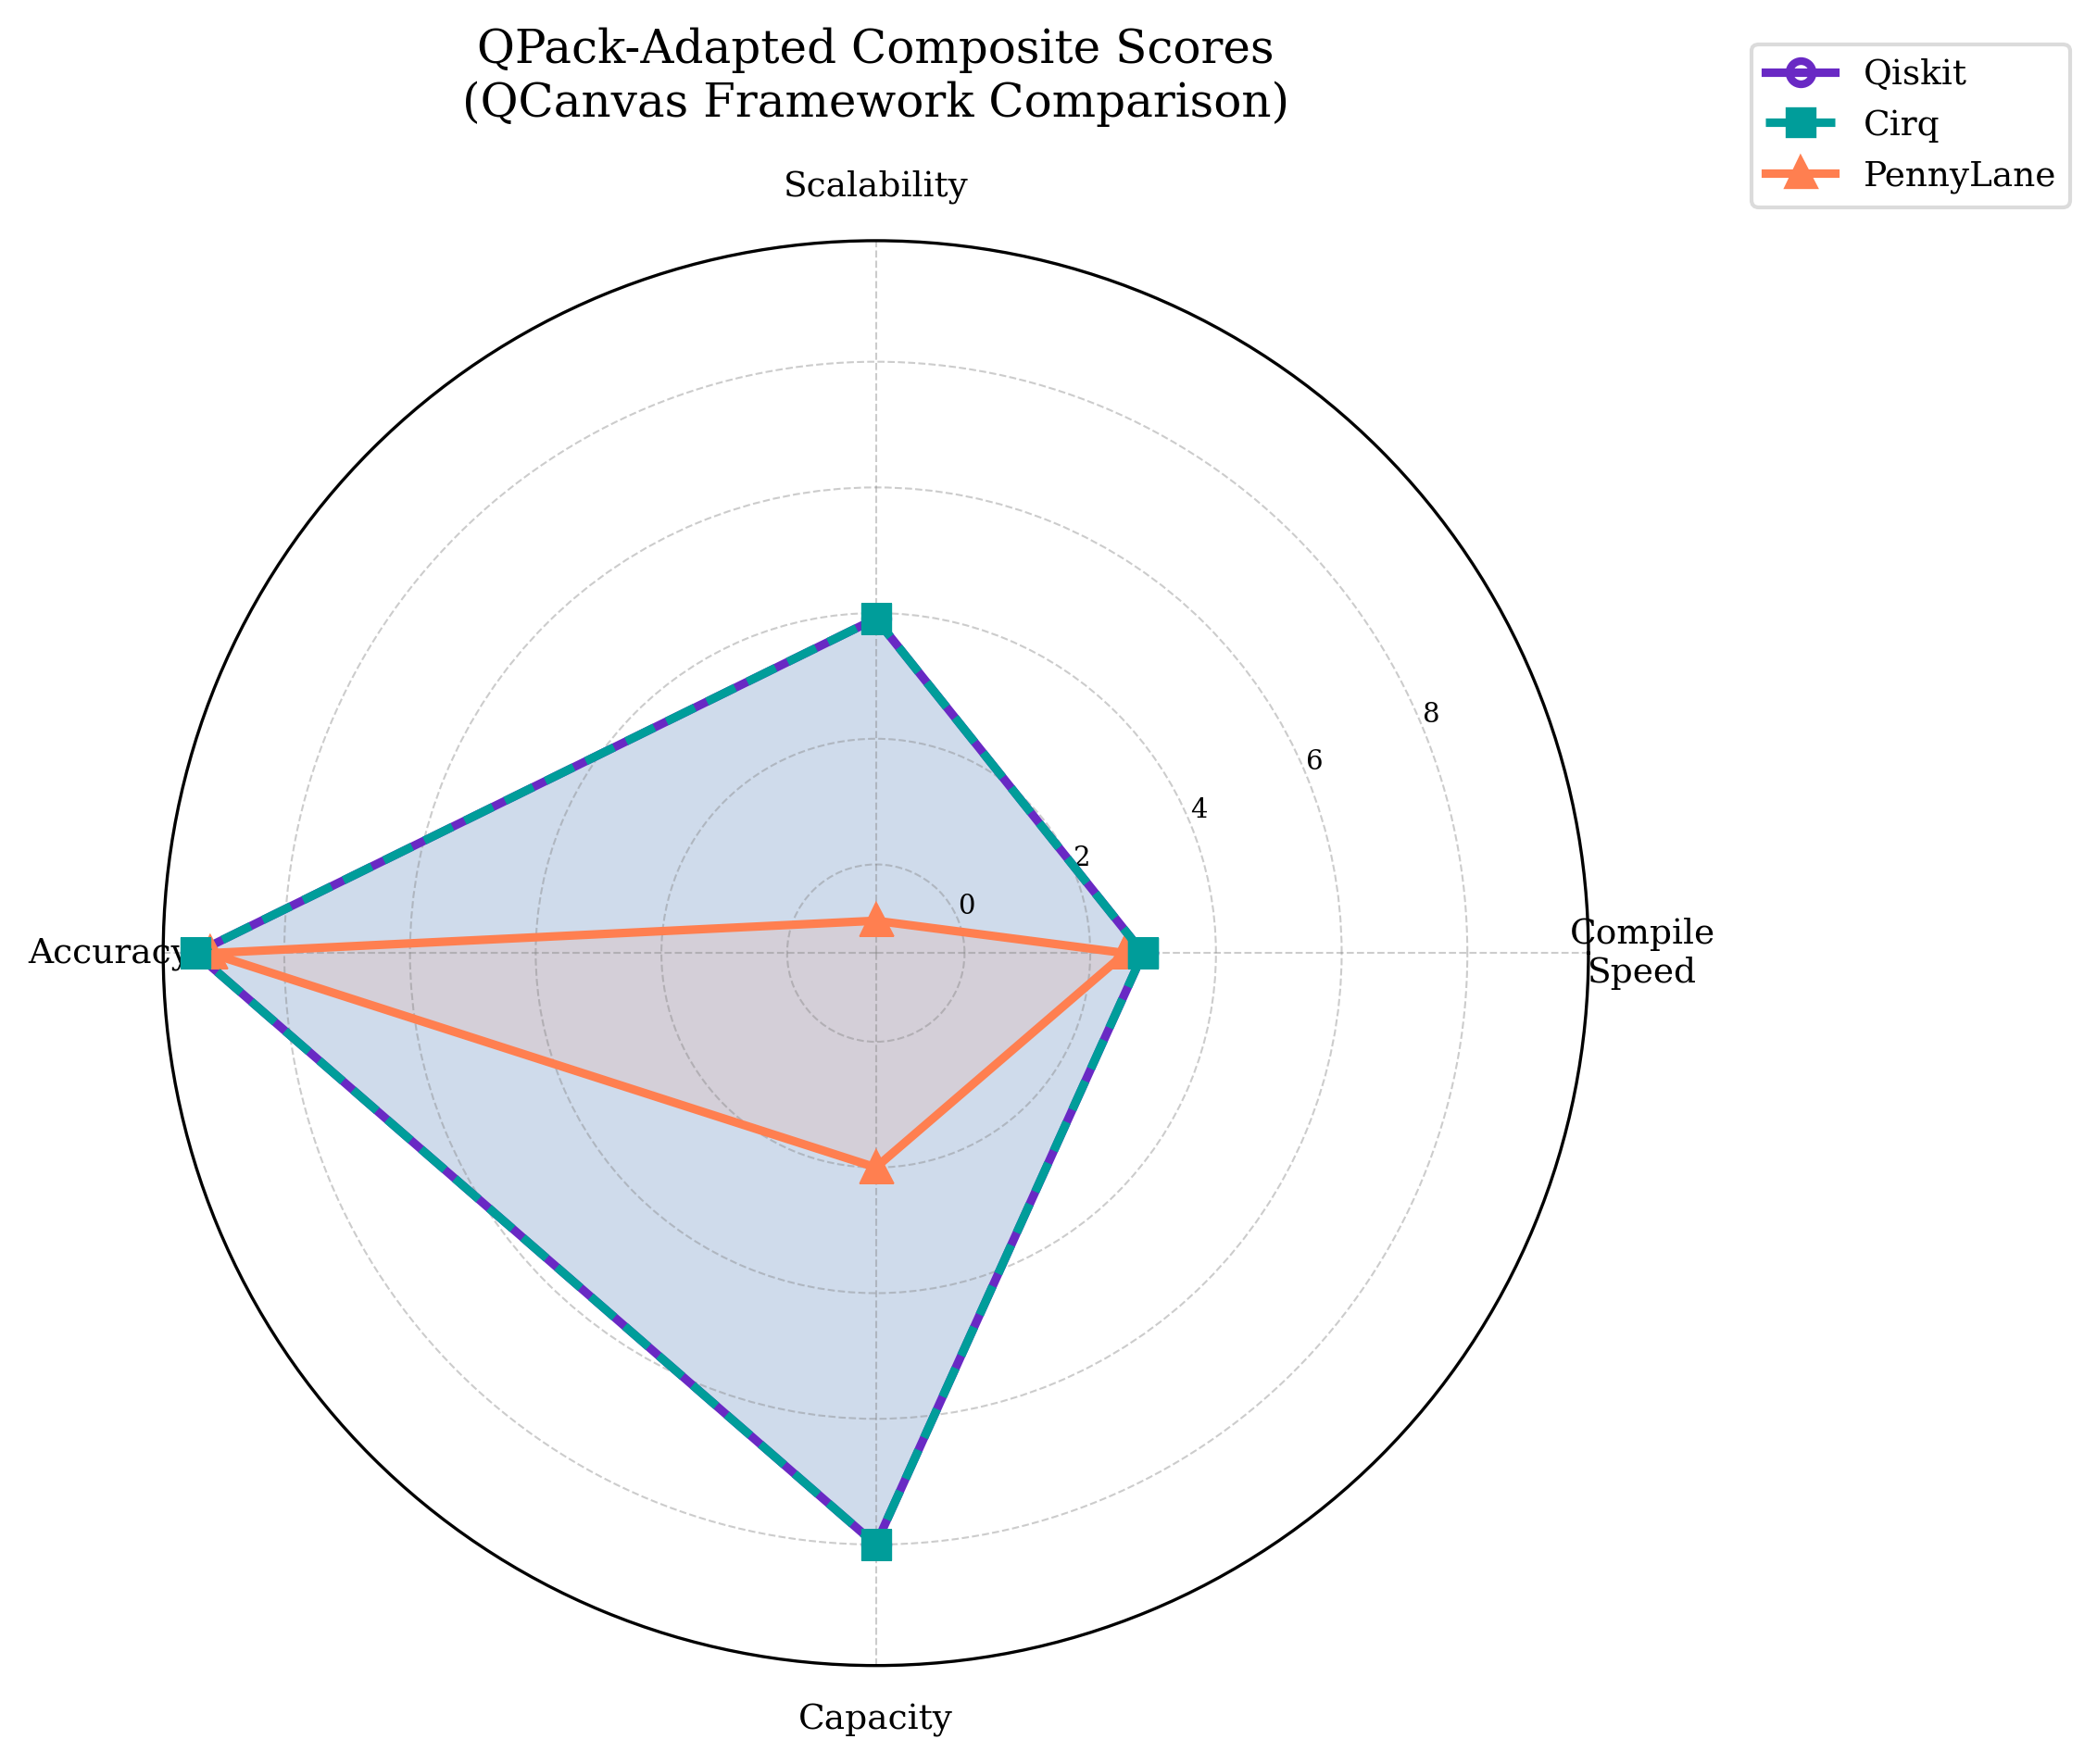
\includegraphics[width=0.75\linewidth]{fig15_qpack_radar}
  \caption{QPack-adapted composite scores radar chart (Fig.~15).}
  \label{fig:radar}
\end{figure}

Table~\ref{tab:qpack} and Fig.~\ref{fig:radar} deliver the clearest
framework ranking.
Qiskit and Cirq are separated by 0.01 in $S_{\text{overall}}$---
effectively tied at 58.80 vs.\ 58.79.
PennyLane scores 9.28, a $6.3\times$ deficit.

Two QPack sub-scores explain PennyLane's position.
$S_{\text{scalability}} = -0.90$ (negative) reflects the Grover's
super-linear gate scaling penalty: the scoring function penalises
super-linear exponents because they render circuits infeasible at
moderate qubit counts.
$S_{\text{capacity}} = 2.00$ versus 8.00 for Qiskit and Cirq reflects
the equivalence failures at scale: PennyLane circuits at 4+ qubits fail
the JSD equivalence check for six of twelve algorithms, reducing its
effective operating range.

All three frameworks achieve QV $= 2048$ ($\log_2 = 11$).
QV is bounded by the simulation backend's effective qubit capacity (11
qubits on this platform), not by framework choice, confirming that
Quantum Volume alone cannot differentiate transpiler quality across
frameworks sharing a common backend.

% ============================================================
%  Section 6 — Discussion  (~1.5 pages)
% ============================================================
\section{Discussion}

\subsection{Framework Selection Guidance}

For NISQ practitioners selecting a framework for oracle, error
correction, or search workloads: Qiskit and Cirq are functionally
interchangeable in circuit-quality terms.
A 0.01 difference in $S_{\text{overall}}$ (58.80 vs.\ 58.79) lies below
any meaningful threshold; selection between them should be based on
ecosystem fit (IBM hardware $\to$ Qiskit; Google hardware $\to$ Cirq)
or team familiarity, not performance.
Both produce constant-depth circuits for oracle algorithms, maintain
statistical equivalence through 8 qubits, and compile with stable,
predictable latency.

PennyLane's advantages lie outside this study's scope.
Its automatic differentiation engine and device-agnostic \texttt{QNode}
abstraction make it the natural choice for variational algorithm research
(VQE, QAOA, QML), where gradient computation across hybrid
quantum-classical loops is the primary concern.
Practitioners using PennyLane for VQE and QML workloads at small qubit
counts ($\leq$2--3 qubits) will observe no equivalence penalty.
The trade-off---larger compiled circuits and JSD$=1.000$ failures at
scale---becomes operationally significant only when the algorithm
requires 4+ qubits and output distributions must be compared with those
from Qiskit or Cirq implementations.

\subsection{The Decomposition Incompatibility Problem}

The JSD$=1.000$ failures reported in Section~5 are not compilation
errors.
PennyLane produces syntactically valid, executable OpenQASM 3.0 circuits
that QSim runs without errors.
The issue is semantic: PennyLane's full decomposition of multi-qubit
oracle gates into primitive two-qubit gates changes the computational
basis in which results are measured at 4+ qubits.
Where Qiskit and Cirq implement a multi-controlled phase operation as a
single structured gate whose output matches the expected oracle behavior,
PennyLane expands the same gate into a sequence of elementary rotations
that, while equivalent in principle, produces a different effective
mapping between input and output basis states when composed with the
algorithm's measurement layer.

This is an underdocumented behavior with serious practical implications.
A practitioner who ports an algorithm from Qiskit to PennyLane at 5
qubits and compares output distributions will observe completely
non-overlapping histograms (JSD$=1.000$) and may incorrectly conclude
their implementation is wrong.
The correct diagnosis is a framework-induced decomposition
incompatibility that is invisible without a common backend.

\subsection{The Unified Pipeline as a Methodological Contribution}

The JSD$=1.000$ findings are discoverable only because all circuits
execute on the same QSim backend.
Had this study used PennyLane's \texttt{default.qubit} alongside
Qiskit's Aer, any divergence would be confounded by the two simulators'
different state-update algorithms, shot-sampling implementations, and
floating-point precision policies.
The QCanvas pipeline removes this confound entirely: a JSD$=1.000$
result in our setup cannot be attributed to the backend; it must be
attributed to the framework's gate-level choices.

\subsection{Hardware Topology and Connectivity Constraints}
\label{sec:hw-topology}

All experiments in this study assume ideal all-to-all qubit connectivity,
corresponding to statevector simulation with no routing overhead.
On real quantum hardware, qubits are arranged in restricted topologies
(e.g., IBM heavy-hex graphs, Google Sycamore grids) and two-qubit gates
can only be applied to physically adjacent qubits.

When a target coupling map is enforced, the transpiler must insert SWAP
gates to route logical qubits to compatible physical qubit pairs;
this routing step is the most computationally expensive and
quantum-error-prone component of the transpilation pipeline.
Comparing Qiskit and Cirq without a coupling map therefore ignores the
primary domain where their transpilers differ most substantially:
Qiskit's SABRE-based router~\cite{li2019tackling} and Cirq's
\texttt{LineSwapRouter} employ fundamentally different heuristic
strategies that produce very different SWAP-overhead profiles depending on
circuit width and hardware topology.
Future work should replicate this benchmark suite on a hardware-constrained
topology (e.g., a 27-qubit heavy-hex map) to characterise the routing
overhead and SWAP insertion penalty for each framework, which we expect
would significantly change the relative gate counts and circuit depths
observed in this study.

\subsection{Limitations}

The following limitations bound the generalisability of these results:

\begin{itemize}
  \item \textbf{Classical simulation only.} All results are from
        statevector simulation.
        Physical hardware validation on NISQ devices---where crosstalk,
        leakage, and device-specific noise profiles dominate---remains
        future work.
        No hardware implications are claimed beyond what the depolarizing
        noise model supports.
  \item \textbf{Simulator mode.} QSim operates in statevector mode;
        density matrix simulation and stabilizer-circuit simulation are
        not evaluated.
  \item \textbf{No hardware coupling map.} All benchmarks assume ideal
        all-to-all connectivity.
        Enforcing a realistic hardware topology would activate SWAP-gate
        insertion and routing heuristics---the most performance-sensitive
        part of any transpiler---which are not evaluated here.
        Gate counts and depths reported in Section~5 therefore represent
        lower bounds on the overhead incurred on physical devices
        (see Section~\ref{sec:hw-topology} for further discussion).
  \item \textbf{PennyLane version pinned at 0.35.1.} Results reflect the
        PennyLane release pinned in the benchmark environment
        (Table~\ref{tab:versions}).
        PennyLane's decomposition strategy may change in future releases.
  \item \textbf{Quantum Volume is structure-implied.} QV is computed from
        circuit structure under a depolarizing model, not from
        heavy-output probability on physical hardware.
        It does not capture real noise profiles (crosstalk, leakage).
  \item \textbf{Algorithm scope.} The 12-algorithm suite is
        representative but not exhaustive.
        Deeper QAOA layers, fault-tolerant codes, and quantum simulation
        circuits are out of scope.
  \item \textbf{Grover scaling extended to 15 qubits (compilation only).}
        To strengthen the power-law extrapolation beyond 5 simulation
        data points, gate-count measurements for Grover's Algorithm were
        extended to 15 qubits via compilation-only runs.
        Statevector simulation was not performed for $n \geq 7$ qubits
        due to memory constraints ($2^{15}$ amplitudes $\approx$256~GB).
\end{itemize}

% ============================================================
%  Section 7 — Conclusion  (~0.5 pages)
% ============================================================
\section{Conclusion}

We introduced a unified benchmarking methodology in which QCanvas
compiles circuits from Qiskit, Cirq, and PennyLane to a common OpenQASM
3.0 intermediate representation for execution on a single QSim
statevector backend, eliminating the simulator confound present in all
prior cross-framework comparisons.
Across 12 algorithms and 6 metric dimensions, Qiskit and Cirq prove
functionally equivalent ($S_{\text{overall}}$ 58.80 vs.\ 58.79), with
selection between them a matter of ecosystem fit rather than performance.
PennyLane exhibits initial super-linear gate scaling for oracle and search
algorithms, with Grover's Algorithm reaching 216 gates at 6 qubits
(a $12\times$ overhead relative to the 18 gates produced by Qiskit and
Cirq), though this transitions to a linear growth regime ($a=0.218$) for
qubits $n \ge 7$.
Most critically, PennyLane's gate decomposition produces JSD$=1.000$
divergence against both other frameworks for six algorithms at 4 or more
qubits, a systematic incompatibility in measurement basis that is
invisible without a common simulation backend.
Future work includes physical hardware validation on NISQ devices,
extension of the suite to fault-tolerant algorithms, and integration of
additional frameworks including Amazon Braket and Stim.


% ---- References ----------------------------------------------
\addcontentsline{toc}{section}{References}
\bibliographystyle{splncs04}   % Springer LNCS bib style
\bibliography{references}

\end{document}
